%\documentclass[a4paper,10pt]{jsarticle}
\documentclass[a4paper,10pt]{jsbook}

\usepackage[dvipdfmx]{graphicx, color}
%\usepackage{folha}
\graphicspath{{image/}}

\usepackage{color}
\usepackage{array}
\usepackage{ascmac}
\usepackage{longtable}
\usepackage{alltt}
\usepackage{graphics}
\usepackage{vpp-nms}
\usepackage{url}
%\usepackage{vpp}
\usepackage{makeidx}
\makeindex

\setlength{\textheight}{42\baselineskip}
\setlength{\footskip}{20pt}

\usepackage{colortbl}

\usepackage[dvipdfmx,bookmarks=true,bookmarksnumbered=true,colorlinks,plainpages=true]{hyperref}

%\AtBeginDvi{\special{pdf:tounicode 90ms-RKSJ-UCS2}}
\AtBeginDvi{\special{pdf:tounicode EUC-UCS2}}

\definecolor{covered}{rgb}{0,0,0}      %black
\definecolor{not-covered}{rgb}{1,0,0}  %red

\setcounter{secnumdepth}{6}
\makeatletter
\renewcommand{\chapter}{%
  \if@openright\cleardoublepage\else\clearpage\fi
  \global\@topnum\z@
  \secdef\@chapter\@schapter}

\renewcommand{\paragraph}{\@startsection{paragraph}{4}{\z@}%
  {1.5\Cvs \@plus.5\Cdp \@minus.2\Cdp}%
  {.5\Cvs \@plus.3\Cdp}%
  {\reset@font\normalsize\bfseries}}
\makeatother

\renewcommand{\sf}{\sffamily \color{blue}}

\newcommand{\syou}{\texttt{<}}
\newcommand{\dai}{\texttt{>}}

%\include{Title}

%\pagestyle{empty}
\usepackage{fancyhdr}
\usepackage{lastpage} 
  \pagestyle{fancy} 
   \let\origtitle\title 
  \renewcommand{\title}[1]
	%{\lfoot{#1}\origtitle{#1}}
	{\origtitle{#1}}

  %\rfoot{\today}
  \lhead{\title}
  \chead{\leftmark}
  \rhead{[\ \scshape\oldstylenums{\thepage}\ / %
      \scshape\oldstylenums{\pageref{LastPage}}\ ]}
  \cfoot{}

\setlength{\textwidth}{\fullwidth}
\setlength{\evensidemargin}{\oddsidemargin}

\begin{document}
% the title page

\title{対象を如何にモデル化するか?\\
%\small{($Revision: 0.2 $ -- \today)}
}
\author{佐原 伸\\
法政大学\\
情報科学研究科
}
%\institute{\pgldk \and \chessnl}
%\date{\mbox{}}
\date{\hfill}
\maketitle

\begin{abstract}
\setlength{\baselineskip}{12pt plus .1pt}
%VDM++言語\cite{CSK2007PP}入門セミナーの演習問題である。
\end{abstract}
%\vspace{-1cm}

\frontmatter % 前付
\tableofcontents
\listoffigures % 図目次
\listoftables % 表目次
\chapter {まえがき}
	独立行政法人情報処理推進機構 (IPA) ソフトウェア・エンジニアリン
グ・センター(SEC) において、ここ数年間にわたって高品質高信頼システムの開発技術に関
して複数の作業部会 (WG) を通して活動を行ってきました。これらの WG の名
称や委員の構成は、状況に応じて変遷してきましたけれども、いわゆるフォー
マルメソッドに基づくソフトウェア開発に関する調査研究ならびに人材育成に
関する活動は一貫して継続してきました。

2010年度以降、フォーマルメソッドに関する入門セミナーないしフォーマルメ
ソッド導入に関するガイダンスセミナーを国内の広島、札幌、熊本、尼崎、名
古屋、東京、盛岡などで開催してきました。この間、セミナー実施経験や受講
者からのアンケート結果などに基づいてセミナー教材の大幅な改訂を行い、
IPA/SEC のホームページ上で「厳密な仕様記述を志すための形式手法入門」と
して公開しています。2012年度からは、改訂版の教材を使用してセミナーを実
施しておりますが、改定前の教材でセミナーを行った都市のなかには改訂版の
教材を用いて再度セミナーを開催したところもあります。

このセミナーは、エンジニア向けと管理者向けに構成を変えて、また、半日コー
ス、一日コース、二日間コースと所要時間も柔軟に組替えられるように工夫し
ました。しかしながら、このセミナーでは、受講者の方々にフォーマルメソッ
ドの概要を伝えることはできても、フォーマルメソッド適用に関する具体的な
手法を理解し習得して頂くには、あまりにも時間が短すぎます。このセミナー
でフォーマルメソッドを代表する一つの手法として取り上げている VDM
(Vienna Development Method) に基づく厳密なシステムの記述に関して、もっ
と具体的に知りたいという受講者の要望も数多く頂きました。

そこで、セミナーで VDM によるシステムの記述の部分を担当している佐原伸氏
に、セミナーで紹介する具体例に関する詳細な副読本としてこの本を執筆して
頂きました。

セミナー教材は、上述のように IPA/SEC のホームページ上で公開されておりま
すので、セミナー受講者でなくても、その教材とこの副読本によってフォーマ
ルメソッド、特に、VDM による厳密なシステム記述に関する基本的な知識と、
システムの厳密な記述の手法に関する理解をえることができます。実のところ、
この副読本は、佐原氏のソフトウェア開発に関する豊富な経験ならびに高い見
識に基づいて、フォーマルメソッドの意義や有用性について実践的な観点から
の説得力ある記述と共に、具体事例を対象として詳細な VDM記述を掲載してお
りますので、フォーマルメソッドの入門書として単独で読んで頂いても十分に
役立つ貴重な書物となっています。

また、IPA/SEC では、フォーマルメソッドのセミナー資料の他にも、「厳密な
仕様記述における形式手法成功事例調査報告書」を公開しています。さらに、
これの報告書に関連して、「厳密な仕様記述入門」という本も作成しました。
これらは、本書の姉妹編とも言うべき有益な資料です。本書と併せてこれらも
ご覧頂くことによって、フォーマルメソッドに基づく高品質高信頼ソフトウェ
アの効率的な開発法に関する理解が深まるとともに、自分たちのところでも実
際にフォーマルメソッドを導入してみようかという気持ちになって頂ければ幸
いです。

 \flushright{荒木 啓二郎}
 \flushright{上流品質技術部会 人材育成WG 主査}
\flushleft{ }
\chapter {はじめに}
	\label{Introduction}
	形式手法で仕様を明確化する技術を教えている時に、
常に問われる「対象を如何にモデル化するか?」を説明するために作成したのが、本ブックレットである。

ここで言うモデル化とは、
システムの仕様に内部矛盾が無いかを検証(正当性検証)し、
ユーザーの要求に合っているかを確認する(妥当性確認)モデルを作成することである。

\section {対象者}
	\index{たいしょうしゃ@対象者}
	以下の対象者を想定して作成した。

	\begin{itemize}
	\item 現場において、システムの品質を改善し生産性を高めたいと考えているプロジェクトのリーダ、開発者の方
	\item 仕様作成とプログラム開発について、ある程度の知見を持っている方 
	\end{itemize}

\section {到達目標}
	\index{とうたつもくひょう@到達目標}

	到達目標は以下の通りである。

	\begin{itemize}
	\item 要求仕様の記述と分析の重要性が理解できていて、第三者に客観的に説明できる。 \\
		特に、厳密な仕様記述が品質向上と生産性向上に寄与することを理解している。
	\item 要求仕様作成のために、「対象を如何にモデル化するか」の手順とその意味が理解できている。
	\item 形式仕様記述言語VDM++を言語マニュアル\cite{SCSK2012PP}等を参照しながら活用すれば、 \\
		小さな実システムの要求仕様を記述する事ができる。
	\end{itemize}

	上記の対象者と到達目標を考慮して、
	実際のシステム開発に流用することができ、
	読者にも知識がある問題について、
	小さな実例をベースに説明を行い、
	形式仕様記述言語VDM++のソースをできるだけ紹介することで、
	具体的イメージを持っていただくことにした。

	ただし、VDM++の言語仕様説明は必要最小限に留めたので、
	VDM++ソース部分を完全に理解するためには、
	VDM++言語マニュアル\cite{SCSK2012PP}を参照していただきたい。

	本書のVDM++ソースは公開されている\footnote{\url{http://sec.ipa.go.jp/reports/20121113.html}}ので、
	いつでもVDMのツールを用いて動かすことができる。
	これがUMLなどの、レビュー以外は検証できず動かないモデル化と大きく異なる点である。

\section {本書の構成}
	\index{ほんしょのこうせい@本書の構成}

	本書は、I\hspace{-.1em}I部構成となっている。

	第\ref{MainBody}部では、対象を如何にモデル化するか?を説明する。

	\ref{WhyFormal}章でなぜ形式手法か?を紹介し、
	\ref{VDMabstract}章で形式手法VDMの概要を説明し、
	\ref{VDMeffect}章でVDM適用の成果を紹介する。

	そして、\ref{How2Intro}章でVDM導入・開発方法・体制の概要を示し、
	\ref{How2MakeModel}章で対象を如何にモデル化するか?を説明する。

	\ref{Conclusion}章でまとめを行い、\ref{Exercise}章で演習問題を示す。

	第\ref{ModelExamples}部では、モデルの具体例を紹介する。
	第\ref{MainBody}部の説明に関連するVDM++モデルのソースとその説明を行なっている。

	\ref{LibraryModel}章は、演習問題の解答例である図書館システムのモデルであり、
	実行不可能な陰仕様
		\footnote{関数・操作のインタフェースと、事前条件及び事後条件しか記述していない仕様を陰仕様と呼ぶ。
		陰仕様は、関数・操作の本体は記述していないが、「仕様」を記述していることになる。}
	と、それを回帰テストするための実行可能な陽仕様
		\footnote{関数・操作の本体が記述されていて実行可能な仕様を陽仕様と呼ぶ。}、
	さらに、やや設計仕様寄りのオブジェクト指向陽仕様としたモデルの例である。
	モデルの理解に必要な、最小限のVDM++文法も説明している。

	\ref{FareModel}章は本文中に出てくる運賃計算モデルであり、
	実システムの10分の1程度の行数でありながら、
	\ref{SpecFramework}節で説明する仕様フレームワークと
	\ref{RegressionTest}節で説明する回帰テストを使った要求仕様の例である。

	\ref{EvolvedExpressReservation}章は、\ref{How2MakeModel}章の
	特急券予約システムを改善したモデルの例であり、
	実用的なシステムを、ある目的のために抽象化して、小さな要求仕様モデルとして記述した例である。

\mainmatter
\part {対象を如何にモデル化するか?}
	\label{MainBody}
\chapter {なぜ形式手法か?}
	\label{WhyFormal}
	形式手法を強く推奨する理由には、
理論的根拠と経験的根拠がある。
以下の節で、それぞれを説明する。

\section {理論的根拠}
	\index{りろんてきこんきょ@理論的根拠}

	形式手法を強く推奨する理論的根拠は、以下の3つである。

\begin{itemize}
\item プログラムは数学系だから
	\index{ぷろぐらむはすうがくけい@プログラムは数学系}

	プログラムは元来、数学的に厳密な体系で定義された一つの数学系である。
	しかも、C++やJavaのプログラムは「検証が困難な数学系
	\footnote{変数への値の代入などの破壊的代入を行うので、
	「同じ条件を与えれば必ず同じ結果が得られ、他のいかなる機能の結果にも影響を与えない」
	という参照透過性を保つことができない。}
	」であることが分かっている。
	これに対して、形式手法は「検証が容易な数学系」をもとにしている。
	したがって、検証しやすい数学系で記述した方が品質を上げやすい。
	


\item 形式手法では、上流工程で仕様を検証可能だから

	要求分析工程
	\index{ようきゅうぶんせきこうてい@要求分析工程}
	\footnote{ユースケース記述などを作成する要求収集(Elicitation)工程の出力を解析し、
	厳密な仕様を記述し、その妥当性確認(validation)と正当性検証(verification)を行う工程。
	本ブックレットでは、要求工学が対象とする工程、あるいは要件定義と称する工程は、要求収集工程と見なす。}
	からプログラミング工程までのどこかで、数学系に変換しなければならない。
	いずれどこかの工程で数学系にするならば、なるべく早い工程、
	すなわち上流工程で数学系にしておいたほうが、
	下流工程から上流工程への手戻りが減り、プログラムの質だけでなく、開発の生産性も向上する。
	そして、形式手法は上流工程での検証を支援する。

	要求分析工程での欠陥修正コストを1とした時の、その他の工程での欠陥修正コストを示したものが、
	図\ref{fig:RelativeCost}である。
		\footnote{Source: Barry Boehm: “EQUITY Keynote Address”, March 19th, 2007}

	\begin{figure}[h]
		\centering
		{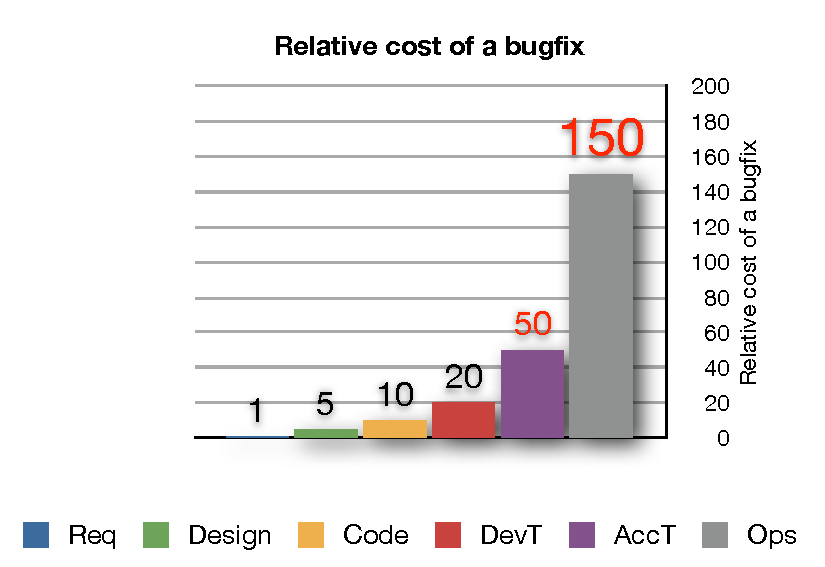
\includegraphics[width=40zw, keepaspectratio] {./Chapter1/image/RelativeCost.pdf}}
		\caption{開発工程別の欠陥修正コスト}
		\label{fig:RelativeCost}
		\index{かいはつこうていべつのけっかんしゅうせいこすと@開発工程別の欠陥修正コスト}
	\end{figure}

	このグラフから分かるように、上流工程での欠陥修正コストは、下流工程のそれの5分の1から150分の1にもなる。

	ここで、横軸のReq, Design, Code, DevT, AccT, Opsは、
	それぞれ要求分析、設計、コーディング、開発テスト、受入テスト、運用の各工程を示している。
	開発テストはシステム開発者によるテスト、受入テストはシステム発注者によるテストである。

\item 旧来の手法では、検証が困難だから

	旧来の手法では、レビュー以外の検証手段が無いため、
	中規模以上のシステムの検証は非常に困難であり、
	大規模システムの検証は不可能といっても良いほどの困難を伴う。

\end{itemize} 


\section {経験的根拠}
	\index{けいけんてきこんきょ@経験的根拠}

	形式手法による仕様記述を行った経験から分かったことは、以下の2点である。

\begin{itemize}
\item 日本語で「正しい」仕様を書くのは「不可能」である

	\begin{itemize}
	\item 曖昧さの排除が困難

		自然言語による仕様では、曖昧さの排除が困難である。

	\item ツールによるチェックが、ほとんど不可能

		自然言語で書かれた仕様を、ツールによってチェックすることはほとんどできない。
		これは、自然言語の文法定義と意味定義が曖昧なことによるもので、
		どのようなツールを作っても、曖昧さを排除することはできない。
		
		これに対し、形式手法で使用される形式仕様記述言語は、
		文法定義・意味定義ともに厳密であり、曖昧な仕様を書くことはできない。

		実際に、\ref{VDMeffect}章で示す成功例では、ツールによる静的検証
		\footnote{モデルを動かさずに検証すること}によって、
		ほとんどの単純ミスを検出し、
		動的検証
		\footnote{モデルを動かして検証すること}によって、
		すべての欠陥を検出し、修正することに成功した。

	\item 仕様の修正に弱い
		\index{しようのしゅうせいによわい@仕様の修正に弱い}

		自然言語仕様の検証は、主としてレビューに頼っているため機械化できない。
		これに対して形式手法は、形式仕様記述言語で書かれた仕様を、機械的に検証する手段を持っている。
		
		\ref{VDMeffect}章で示す成功例では、「仕様修正に強い」形式手法の利点が、品質向上と検証工数削減に大いに役立った。
		
	\item その場で「文法」を考えなければならない

		日本語で仕様を書ききれなくなり、if文などを使った擬似コード的な仕様を書くことが多く、
		擬似コードの文法
		\index{ぎじこーどのぶんぽう@擬似コードの文法}
		を考えている時間が馬鹿にならない。
		すなわち、仕様を書く際に、仕様の意味ではなく、文法に注意が向いてしまい、
		肝心な「意味を考える」ことがおろそかになってしまう。

	\end{itemize} 

\item 形式手法の方が技術移転や蓄積が容易である

	\begin{itemize}
	\item 日本語による意思疎通は難しい
		\index{にほんごによるいしそつう@日本語による意思疎通}


		日本語仕様は、開発者間のコミュニケーションを経るたびに、
		一種の伝言ゲームになってしまい、当初の意味がずれていくことが多い。
		打ち合わせなどで「あれって、こういう意味じゃないの」というような議論が起こることが多ければ、
		それは、自然言語の曖昧さによって意思疎通がうまくいっていない事の証である。

	\item 仕様記述言語を読むのは容易である
		\index{しようきじゅつげんごをよむのはようい@仕様記述言語を読むのは容易}

		自然言語仕様であろうが、形式仕様であろうが、仕様を書くことは難しい。
		しかし、記述された仕様を読むことは、形式仕様記述言語の場合、容易である。
		それは、非形式的な図形言語UML1.xより容易であり、UML2.0より遙かに簡単である。
		\index{UML@UML}

	\item フレームワークやライブラリの構築が容易である
		\index{ふれーむわーくやらいぶらりのこうちくがようい@フレームワークやライブラリの構築が容易}

		形式仕様記述言語は、プログラミング言語などと同じように、
		フレームワークやライブラリの構築が容易であり、
		再利用性や保守性に優れている。

	\item 業務知識の蓄積も容易である
		\index{ぎょうむちしきのちくせい@業務知識の蓄積}


		ExcelやWordによる自然言語仕様と異なり、形式仕様記述言語の仕様は通常テキストファイルであり、
		プログラミング言語と同じように、版管理や構成管理ツールと連動して容易に管理できるため、
		業務知識をいったん形式仕様記述言語で記述できれば、
		それを、再利用・保守可能な業務知識として、蓄積していくことが容易である。
	
	\item 仕様を「動かしてみる」ことができるので、理解しやすい
		\index{しようをうごかす@仕様を動かす}
		形式手法は、形式仕様を動かす(実行する\footnote{仕様アニメーションという}、
		モデル検査する、証明する)ことが可能で、
		動かない旧来手法より理解することが容易である。
	\end{itemize} 
\end{itemize} 


\section {日本語仕様の曖昧さの例}
	\index{にほんごしようのあいまいさのれい@日本語仕様の曖昧さの例}

	この節では、著者が出会ったことのある、日本語仕様の曖昧さの例を示す。

\subsection {図書館の本}
	\addcontentsline{toc}{section}{図書館の本}
	\index{としょかんのほん@図書館の本}

	図書館のシステムを考えた場合、以下の2つの文に出てくる「本」は同じものを意味しているだろうか?

\begin{itemize}
	\item 題名で本を検索する
	\item 本を図書館の蔵書として追加する
\end{itemize} 

	この2つの「本」は同じ場合もあるが、
	普通は、異なるものを指す。

	「題名で本を検索する」場合の「本」は、多くの場合、ある著者が書いたある題名の「本」を指す。
	この「本」は抽象的な概念で、例えばこの「本」が1000部出版されているとしても、我々は「ひとつの本」として認識している。

	しかし、図書館の蔵書に追加する「本」はそうではない。
	これは物理的な1冊の本であり、抽象的な「本」が1000部出版されていれば、こちらの「物理的な本」は1000冊存在する。

	日本語による仕様記述では、このように区別すべき用語が同じものとして記述されたり、
	同じ意味の用語が別の言葉で記述されて曖昧さが混入し、開発者同士のコミュニケーションが混乱し、
	結果として、作業の手戻りの多発による生産性の低下と品質の低下を招く。

	詳細は、\ref{LibraryModel}章を参照していただきたい。

\subsection {特急券予約システム}
	\addcontentsline{toc}{section}{特急券予約システム}
	\index{とっきゅうけんよやくしすてむ@特急券予約システム}

	ここでは、筆者が実際に遭遇した、鉄道会社Aの特急券予約システムの問題点を紹介する。

	問題の発端は、クレジットカード会社の都合で、
	特急券予約システムに使用していたクレジットカードを変更せざるを得なくなり、
	特急券予約システムの設定を変更しようとしたところから始まった。

	以下は、鉄道会社Aサポートセンターとの問答である。
	\footnote{実際にあった事例をかなり省略している。}

\begin{enumerate}
\item 客(すなわち筆者)は、おサイフケータイ(鉄道会社B)で特急券予約システム(鉄道会社A)を使っていた。
\item 会社Cクレジットカードが廃止になり会社Dクレジットカードに変更して下さいとの連絡があった。
\item 鉄道会社Aサポートセンターに電話したところ、
	おサイフケータイの登録クレジットカードを変更すれば、2日後には特急券予約システムが使えますとのことだった。
\item おサイフケータイの設定でクレジットカードを変更し、2日後に使おうとしたが、特急券が予約できなかった。

\item 予約できなかったので鉄道会社Aサポートセンターに電話した

	\begin{description}
	\item [客]「クレジットカードを変更したら、予約できないんですが?」
	\item [鉄道会社A]「カードを変更したら、新規に特急券予約システムを契約して下さい。」
	\item [客]「クレジットカード変更前に予約した特急券に引き換えようとしたらできないのですが?」
	\item [鉄道会社A]「カードで引き替えできるようになったので、それで引き換えて下さい。暗証番号はカードのものを使って下さい。」
	\item [客]「カードの暗証番号って、何ですか?」
	\item [鉄道会社A]「クレジットカードの暗証番号です。」
	\end{description}

\item 旅行当日のT駅での問答

	\begin{description}
	\item [客]「クレジットカードで特急券に引き換えできないんですが?」
	\item [鉄道会社B]「会員証でやってみて下さい。」
	\item [客]「会員証でもできないんですが?」
	\item [鉄道会社B]「変ですねー、こちらでやってみましょう。駄目ですねー...」
	\item [客]「ひょっとして、古いクレジットカードでは駄目ですか?」
	\item [鉄道会社B]「あ、できましたね。はい、切符です。」
	\end{description}
\end{enumerate}

	上記のやり取りで、何が起こっていたかを正確に理解できる方は居るだろうか?
	理解できるはずはない。
	鉄道会社A側の用語の使い方が適切ではないので、
	鉄道会社Aサポートセンターの要員も、T駅の鉄道会社Bの駅員も事態を正確に把握できなかったのだから。

その後、手元にある特急券予約システム関係のカード類と、インターネット上の情報と、
鉄道会社Aサポートセンターへの何回かの電話によって、幾つかの用語の定義、すなわちカードの種類が判明した。

すなわち、

\begin{itemize}
	\item 予約会員証 (変更前、変更後)、クレジットカード(変更前、変更後)
	\item おサイフケータイ
		\footnote{ここでは、スマートカードとして特急券を予約する機能だけに着目する。}
	\item ICカード、予約カード
\end{itemize} 

このうち、ICカードはおサイフケータイで予約する場合には関係ないカードであることが判明した。
また、予約カードも鉄道会社Aのカードであり、
おサイフケータイ(鉄道会社B)から特急券予約システムする場合には関係ないことも判明した。

これらを反映して、最初の鉄道会社A側とのやり取りを、正確な用語で記述すると以下のようになる。

\begin{enumerate}
\item 予約できなかったので鉄道会社Aサポートセンターに電話した

	\begin{description}
	\item [客]「クレジットカードを変更したら、予約できないんですが?」
	\item [鉄道会社A]「クレジットカードを変更したら、新規に特急券予約システムを契約して下さい。」
	\item [客]「クレジットカード変更前に予約した特急券に引き替えようとしたらできないのですが?」
	\item [鉄道会社A]「予約会員証で引き替えできるようになったので、それで引き換えて下さい。
			暗証番号はクレジットカードのものを使って下さい。」
	\end{description}

\item 旅行当日のT駅での問答

	\begin{description}
	\item [客]「変更後のクレジットカードで特急券に引き換えできないんですが?」
	\item [鉄道会社B]「予約会員証でやってみて下さい。」
	\item [客]「予約会員証でもできないんですが?」
	\item [鉄道会社B]「変ですねー、こちらでやってみましょう。駄目ですねー...」
	\item [客]「ひょっとして、変更前のクレジットカードでは駄目ですか?」
	\item [鉄道会社B]「あ、できましたね。はい、切符です。」
	\end{description}
\end{enumerate}

この記述は、VDM++という形式仕様記述言語を使って、前記の問答に関わる仕様(モデル)
\footnote{詳細は、\ref{How2MakeModel}章と、\ref{EvolvedExpressReservation}章を参照のこと。}
を書き、
最初の問題発生から3ヶ月かかって、問題を解決した後に記述したものである。


\subsection {応当日}
	\addcontentsline{toc}{section}{応当日}
	\index{おうとうび@応当日}

以下は、証券会社用のパッケージソフトウェアを作成していた際、
「信用取引の決済日」の定義を聞いた時に回答として得た説明文章である。

\begin{itemize}
	\item 信用取引の決済日(期日)を得る。

	弁済期限とは、信用建玉に対して当社がお客様に信用を供与する期限をいいます。
	弁済期限は、現在のところ6ヶ月のみを取扱っています。
	弁済期限が6ヶ月であるということは、
	信用建玉の建日(信用建玉が約定した日)の6ヶ月目応当日が信用期日となり、
	この日を超えて建玉を保有することは法律で禁じられています。
	信用期日が休日の場合には、直近の前営業日が信用期日となります。
\end{itemize} 

直ちに生じる疑問は、以下のようなものであろう。

\begin{itemize}
	\item 弁済期限と決済日と信用期日との関係は?
	\item 応当日とは何か?
\end{itemize} 

弁済期限と決済日と信用期日との関係を質した所、直ちに回答が得られた。
すなわち、これらは同一である。

応当日については、何回かのやり取りの後、以下の回答が得られた。

普通の日本語で書くと分かり難くなるので、
やや形式化した日本語で応当日を「曖昧に」定義すると、以下のようになる。

\begin{verbatim}
現在日をy年m月d日としたとき、nヶ月後の応当日とは、y年m+n月d日のこと。

ここで、m+n >= 13 ならば、
   年候補Yをy + (m+n - 1) div 12とし、
   月候補Mをm+n mod 12として、
      Mが0ならば、Mは12、
      Mが0以外ならば、Mをそのまま使って、
Y年M月d日が応当日である。
ここで、divは整数の除算、modは整数除算の余りを得る演算子である。
\end{verbatim}

この日本語仕様には、まだ、以下の問題が残っている。

\begin{enumerate}
\item たとえば信用建玉の建日が8月31日だと、応当日は翌年2月31日になってしまうのだが、
	そのとき2月28日あるいは2月29日にするのか3月1日にするのかの記述がない。
\item 応当日から月初日まですべて休日の場合、前月の営業日にしてよいのかどうかの記述がない。
\end{enumerate}

この疑問は、証券業務の専門家に質問したところ、半日ほどで回答を得た。

\begin{itemize}
	\item 月末日を越えたら、月末日に最も近いその月の営業日。
	\item 応当日が休日で、前営業日が前の月の場合、その営業日が応当日になる。
\end{itemize} 

以上のように、「信用取引の決済日を得る」という証券業務にとっては基本的な用語すら、
同じ事を表す複数の言葉が存在し、定義が曖昧で、
ある程度の仕様分析を行った後、
証券業務の専門家に質問しても答えを得るのに半日以上を要して
ようやく正しい仕様を理解できた。

しかも、応当日の年や月を求める計算は、日本語で記述し理解するには複雑すぎる。

これでは、生産性と品質が悪くなるはずである。

\chapter {形式手法VDM概要}
	\label{VDMabstract}
	本章では、形式手法の概要と本ブックレットで使用するVDMについて説明する。

\section{形式手法VDMとは?}
	\label{WhatIsVDM}
	\index{けいしきしゅほうVDMとは@形式手法VDMとは?}
VDMはVienna Development Methodの略であり、
1960年代から1970年代にIBMウィーン研究所で開発され、
IBMの各種プログラミング言語の仕様記述に使用された。

その後、汎用の仕様記述言語として拡張され、
1996年に、その仕様記述言語VDM-SL\cite{SCSK2012SL}
が世界初のISO標準(ISO/IEC 13817)仕様記述言語になった
	\index{ISOひょうじゅん@ISO標準(ISO/IEC 13817)}
形式手法の元祖である。


特徴としては、以下がある。

\begin{itemize}
	\item 厳密に定義された仕様記述言語VDM-SL, VDM++, VDM-RTを持つ
	\item 制約条件(不変条件、事後条件、事前条件)の記述が可能である
	\item 証明手法がある\footnote{証明手法は初心者には難しいため、本書では説明を省略した。}
	\item 産業界の実用のために拡張された
\end{itemize} 

\section{VDM++とは?}
	\label{WhatIsVDMPP}
	\index{VDM++とは@VDM++とは?}

VDM++\cite{Kyushu2016PP}は、1993年に、欧州連合ESPRIT計画のAFRODITEプロジェクトで、
VDM-SL\cite{Kyushu2016SL}をオブジェクト指向拡張したオブジェクト指向形式仕様記述言語である。

オブジェクト指向構文以外に、関数型言語構文を持ち、
C++やJavaなどと同じく構造化言語の構文も持っている。

VDMToolsとOverture Toolsという2つのVDM++支援ツールがあり、
それらを用いて、以下の様な仕様の検証が可能になった。

\begin{itemize}
	\item 構文チェック、型チェック、仕様アニメーション(仕様のシンボリック実行)
	\item 仕様アニメーションによる組合せテストおよび回帰テストと、テストのコードカバレージ表示
	\item 証明課題
		\index{しょうめいかだい@証明課題}
		\footnote{証明課題が全て証明できれば、モデルに内部矛盾は無いと主張できる。}
		生成機能を使った、証明課題レビュー
\end{itemize} 

VDMToolsは、C++とJavaの生成機能がある。

\section{なぜVDMを選択したか?}
	\label{WhyVDM}
	\index{なぜVDMをせんたくしたか@なぜVDMを選択したか?}

\subsection{形式手法の種類}
	\index{けいしきしゅほうのしゅるい@形式手法の種類}

形式手法には主なものとして、モデル規範型、性質規範型、モデル検査がある。
この中で、現場の技術者に理解しやすくシステム全体を仕様化できるので、
モデル規範型VDMを採用した。
実際に\ref{VDMeffect}章で紹介するシステムでは、
3ヶ月の学習と仕様記述の試行を経て、実用開発を行うことができた。

モデル規範型には、他にもB, event-B, Z, RAISEといった有用な手法があるが、
いずれも、「証明を前提」としているため、
開発現場で適用する「最初の形式手法」としては、不適切と判断したのである。

性質規範型の手法としては、CafeOBJやMaudeなどがあるが、
VDMより1段階抽象度が高く、これも「最初の形式手法」としては、不適切と判断した。

モデル検査手法にはSPINやSMVがあるが、
モデル検査用仕様記述言語は、検証効率を上げるため、
システムの振舞を表す部分の一部だけを仕様記述するため、
データ構造などを含むシステムの他の側面をほとんど記述することができない。
すなわち、システム全体の仕様を記述することはできず、
ある側面からの検証にとどまり、
かつ、開発現場に適用するには3年程度の試行期間が必要と思われ、
「最初の形式手法」としては不適切と判断した。

\subsection{形式手法の検証方法とツール}
	\index{けいしきしゅほうけんしょうほうほうとつーる@形式手法の検証方法とツール}

形式手法の検証方法としては、証明・モデル検査・仕様アニメーションの3つがある。

証明はRAISEを支援するRAISE Toolや、event-Bを支援するRodinがあるが、
最低でも5年程度の学習期間が必要と判断して、
「最初の形式手法」としては採用しなかった。

モデル検査は、ツールを使用することにより、
教科書的な簡単な問題は、簡単に検証することができる場合があるが、
エラーが見つかった場合の、原因の特定などに難しいところがあり、
「最初の形式手法」としては採用しなかった。

結局、VDMを使用するVDMToolsが、仕様アニメーションを使用しているので、
プログラムテストと同じ感覚で使用することができるため、
開発現場の技術者の「最初の形式手法ツール」として最適だと判断した。

\subsection{VDMの参考文献}
	\label{VDMref}
	\index{VDMのさんこうぶんけん@VDMの参考文献}
VDM++\cite{Kyushu2016PP}は、
1970年代中頃にIBMウィーン研究所で開発されたVDM-SL\cite{Kyushu2016SL}を拡張し、
さらにオブジェクト指向拡張した形式仕様記述言語である。

VDM++の教科書としては\cite{Sakoh2010}がある。

VDM++を開発現場で実践的に使う場合の解説が\cite{Sahara2008}にある。



\chapter {VDM適用の成果}
	\label{VDMeffect}
	VDMの海外での適用事例は、
	\index{VDMのかいがいでのてきようじれい@VDMの海外での適用事例}
IBMでの多くのプログラミング言語開発、旧ソ連の100万行以上の仕様で記述された衛星システム、
VDM++からC++を生成したオランダの世界最大の花市場オークションシステムなどがある。

日本での適用事例には、表\ref{VDMeffectTable}がある。
	\index{VDMのにほんでの適用事例@VDMの日本での適用事例}

\begin{table}[h]
	\caption[VDMによる仕様作成の成果]{VDMによる仕様作成の成果}
	\index{VDMによるしようさくせいのこうか@VDMによる仕様作成の成果}
	\label{VDMeffectTable}
	\begin{center}
		\setlength{\tabcolsep}{3pt}
		\begin{tabular}{|c|c|c|r|r|r|r|} \hline
			開発組織 & 対象システム & 適用工程 & 仕様規模 & 欠陥数 & 生産性 & 開発期間   \\ \hline\hline
			日本フィッツ& 証券業務 & 実システム & 3+3万行 & 0 & 2.5倍 & 45\%  \\ 
			現SCSK &  & UseCase & 仕様+テストケース &  &  &   \\ 
			 &  & 要求仕様 &  &  &  &   \\ \hline
			フェリカネットワークス & おサイフケータイ &  実システム & 7.4+6.6万行 & 0 & 2倍 & 85\% \\ 
			 & ファームウェア &  API外部仕様 & 仕様+テストケース &  &  &   \\ \hline
			産業技術総合研究所 & 鉄道 & 既存システム & 0.75+80万行 &  従来仕様書の & &   \\ 
			オムロン & 駅務システム & 厳密仕様 & 仕様+テストケース & 欠陥発見数 & &   \\ 
			 &  & 作成実験 &  & (29) & &   \\ \hline
		\end{tabular}
	\end{center}
\end{table}

表\ref{VDMeffectTable}では、生産性と開発期間の比較は、
COCOMO81\cite{Boehm81}による見積りと実績値の比較で行った。
生産性のカラムは、見積もりに対して実績値が何倍になったかを示し、
開発期間のカラムは、見積もりに対して実績値が何\%であったかを示している。

仕様規模のカラムは、m + n という形式で、注釈抜きのVDM++ソース行数を表していて、
mの部分は仕様本体、nの部分はテストケースの行数を表している。

以下に、各システムの概要を述べる。

\section{日本フィッツの事例}
	\label{JFITS}
	\index{にほんふぃっつのじれい@日本フィッツの事例}

証券会社バックオフィスシステム
	\index{しょうけんがいしゃばっくおふぃすしすてむ@証券会社バックオフィスシステム}
用パッケージソフトウェアの2つのサブシステムにVDM++仕様を適用した。
最初に手がけたサブシステムは識別子に英語を使用したが、
2つ目のサブシステムでは、VDMToolsを修正して国際語化し、日本語識別子と日本語文字列を使用したVDM++仕様を作成した。
	\index{こくさいごか@国際語化}
	\index{にほんごしきべつし@日本語識別子}

開発チームは証券業務の知識がなく、仕様が曖昧なまま開発するのは危険と考え、
UseCaseレベルの要求仕様記述をVDM++を用いて行い、
回帰テストのテストケースもVDM++で記述し、
仕様の検証をVDMToolsの仕様アニメーション機能(シンボリック仕様実行)で行った。
回帰テストのコードカバレージをVDMToolsで計測し、
リリース時には95\%以上のカバレージを達成した。

開発チームのうちの2人がVDM++による記述を行ったが、
2人ともVDM++の知識はあったものの、実際にVDM++を業務として使うのは初めてだった。
プログラマもJavaとC++の知識はあったものの、実業務に使うのは初めてであった。

表\ref{VDMeffectTable}には、VDM++で開発した3000行あまりのライブラリの開発工数も含まれていて
、ライブラリを除くアプリケーション開発自体の生産性はさらに高いが、
ライブラリ開発とアプリケーション開発の工数を分離して計測する時間的余裕は無かったため、
ライブラリ開発がどの程度の割合を占めたかの正確なデータは残っていない。

\section{フェリカネットワークスの事例}
	\label{FeliCa}
	\index{ふぇりかねっとわーくすのじれい@フェリカネットワークスの事例}

以前のおサイフケータイ・ファームウェアの開発
	\index{おさいふけーたいふぁーむうぇあのかいはつ@おサイフケータイ・ファームウェアの開発}
で、仕様の曖昧さのため非常に苦労したため、
VDM++で仕様を書き、検証することになった。

日本フィッツの開発者をコンサルタントとし、
証券業務仕様の記述で用いた仕様記述フレームワーク
	\footnote{仕様記述フレームワークは、仕様のどの部分に何を書くかを定めた規則である。
	詳しくは、\ref{SpecFramework}節に説明する。}
を流用して、
予定通り開発を終了し、現在に至るまで欠陥が発生していない。

開発者に形式手法の知識はなかったため、
中心となる技術者にVDM++を教育し、
仕様記述フレームワークとその使用例を開発し、
それを元に、他の技術者が仕様を作成した。

API外部仕様は、今までどおりの日本語仕様と、VDM++仕様の両方を記述し、
矛盾する場合はVDM++仕様を優先することとした。

なお、本システムの対象はモバイルFeliCaチップであるが、
	\label{FeliCaちっぷ@FeliCaチップ}
本システムの後、EdyカードのFeliCaチップ開発にもVDM++が使用され、
	\label{Edyかーど@Edyカード}
本システムと同等以上の成果を上げた。
このシステムでは、従来型の日本語仕様は作成せず、
日本語識別子を使ったVDM++仕様のみを作成した。

また、セキュリティ強化版のFeliCaチップ
	\index{せきゅりてぃきょうかばんのFeliCaちっぷ@セキュリティ強化版のFeliCaチップ}
	\footnote{IC RC-SA00/1 SeriesとRC-SA00/2 Series}
	\label{FeliCaちっぷ@FeliCaチップ}
	\index{IC RC-SA00}
開発にもVDM++が使用され、
情報セキュリティ評価基準の国際標準であるコモンクライテリア(ISO/IEC 15408)において、
	\index{ISO/IEC 15408}
組み込みソフトウェアを搭載した非接触ICカードチップとして
	\index{ひせっしょくICかーどちっぷ@非接触ICカードチップ}
世界で初めて評価保証レベルEAL6+認証を取得した。
	\index{EAL6+}


\section{オムロンの事例}
	\label{OMRON}
	\index{おむろんのじれい@オムロンの事例}

駅務システム
	\index{えきむしすてむ@駅務システム}
は社会インフラとして高い信頼性が求められているが、
従来の仕様書は、今や、理解することや保守あるいは再利用が非常に困難となってきたため、
既存仕様をVDM++で書き換える実験を行った。

結果として、従来型仕様書の不備を29件発見し、
暗黙知
\footnote{ここで言う暗黙知は、担当者の一部だけが知っている業務知識で、明文化されていないものを指す。}
がVDM++で1400行相当発見され、
鉄道会社共通の仕様もVDM++で1400行発見された。

開発者は「暗黙知は仕様の欠陥であると認識した」と述べている。

検証は、産業技術総合研究所の検証サーバー「さつき」を利用し、
64コアCPUのマシンで実テストデータ80万件で5日間実行した。
このテストの実行速度は、実機の10分の1から20分の1であった
\footnote{SEC特別セミナーアーキテクチャ指向エンジニアリングと形式手法における以下の発表資料による。
幡山五郎、大崎人士、相馬大輔、Nguyen Van Tang 著、
上流工程大規模テストのための技術開発
~組込みシステム開発のフロントローディング化~,
2011年7月5日
}。





\chapter {VDM導入・開発方法・体制の概要}
	\label{How2Intro}
	本章では、VDMを如何に導入し、どのような開発方法・体制を採用したかを述べる。

\section{VDMの教育}
	\label{Education}
	\index{VDMのきょういく@VDMの教育}

	日本でVDMの導入に成功した表\ref{VDMeffectTable}の事例で行われた教育の内容を表\ref{VDMEducation}に示す。

\begin{table}[h]
	\caption[VDMの教育]{VDMの教育}
	\index{VDMのきょういく@VDMの教育}
	\label{VDMEducation}
	\begin{center}
		\setlength{\tabcolsep}{3pt}
		\begin{tabular}{|p{11zw}|p{5zw}|p{4zw}|p{10zw}|p{9zw}|p{12zw}|} \hline
			組織 & セミナー & 教材 & コンサルティング & 受講者 & 備考 \\ \hline\hline

			日本フィッツ & 4日間 & 英語 & 
				形式手法知識を持った要員とオブジェクト指向分析・設計手法(OOA/OOD)専門家の要員が相談 & 
				平均年齢50歳弱 & VDM記述予定者の3分の1(2人)は英語で脱落 \\ 
				(現SCSK) & & & & 形式手法知識4人有 & \\ 
				 &  & & & ソフト工学知識有 & C++, Java, 形式手法について、実践経験無 \\ 
				 &  & & & 業務知識無 & \\ \hline

			フェリカネットワークス & 4日間 &  日本語 & 3ヶ月/週1回 & 平均年齢20歳代 & \\ 
				 & & & & 形式手法知識無 & \\ 
				 & & & & ソフト工学知識無 & \\ 
				 & & & & 業務知識有 & \\ \hline
			産業技術総合研究所 & 無し & 日本語 & 最初は無し & 平均年齢30歳代 & 周囲に形式手法経験者多数 \\ 
				オムロン & 自習 & 参考文献 \cite{Sakoh2010} \cite{Sahara2008} & その後、3ヶ月/週1回 & 形式手法知識1人有 & \\ 
				 & & & & ソフト工学知識無 & \\ \hline
		\end{tabular}
	\end{center}
\end{table}

海外の形式手法使用事例でも、形式手法の初期教育は約1週間であり、
その後3ヶ月ほど形式手法の専門家によるコンサルティングを経て、
成功している事例がほとんどであり\cite{SEC2012FMREPORT}、
日本での成功例の場合と教育方法・手順はほとんど同じである。

なお、日本フィッツの場合は開発チーム全員がVDMセミナーを受講したが、
フェリカネットワークスは仕様記述フレームワーク作成予定者のみVDMセミナーを受講した。

\section{仕様記述}
	\label{Specification}
	\index{しようきじゅつ@仕様記述}

	VDM++を使って、仕様記述者がそれぞれ独自の仕様記述を行った場合、
	仕様の可読性や再利用性、保守性などが損なわれることが予想されたので、
	仕様記述のフレームワークを定め、仕様ライブラリを作成した。

\subsection{仕様記述フレームワーク}
	\label{SpecFramework}
	\index{しようふれーむわーく@仕様記述フレームワーク}

仕様記述フレームワークは、仕様のどの部分に何を書くかを定めた規則である。
どのように書くかを示すテンプレートとして提示したり、
関連する仕様ライブラリを使用するよう指示する部分もあるが、
多くは、日本語文で定めた規則である。

仕様記述のためのフレームワークを作成した目的は以下の通りである。

	\begin{itemize}
	\item 仕様の可読性、再利用性、保守性の向上
	\item 仕様記述者のVDM技術レベルと仕様の階層を対応させ、VDM初級者でも仕様記述を行えるようにする
	\item DBインターフェースの隠蔽を行い、RDBによる実装を行いやすくする(日本フィッツ事例(\ref{JFITS}節)の場合)
	\item 実装側フレームワークと対応させ、仕様とプログラムの対応関係が分かりやすいようにする(日本フィッツ事例の場合)
	\end{itemize}

\subsubsection{仕様記述フレームワークの概要}
	\index{しようふれーむわーくのがいよう@仕様記述フレームワークの概要}

	\paragraph{仕様記述の対象}
		\index{しようきじゅつのたいしょう@GUIの捨象}

	日本フィッツ事例(\ref{JFITS}節)では、ユースケース・レベルの業務論理(Business Logic)を仕様記述の対象とした。
	
	フェリカネットワークス事例(\ref{FeliCa}節)では、ファームウェアのAPI仕様を仕様記述の対象とした。

	\paragraph{GUIの捨象}
		\index{GUIのしゃしょう@GUIの捨象}
	仕様記述フレームワーク作成では、GUIは捨象して記述しなかった。

	これは、日本フィッツ事例の場合、サーバー側のユースケース・レベルの仕様を記述することが一番重要であり、
	クライアント側のGUIは、ユースケース・レベルの仕様記述とかなりの部分が重複するため、
	従来通りの画面仕様を中心とした仕様を使った。

	GUIを除くクライアント側の仕様も、記述するための仕様記述フレームワークは試作したが、
	サーバー側のユースケース・レベル仕様との重複が多く、記述工数と比較して効果が薄いと判断し、
	記述しなかった。
	
	フェリカネットワークス事例の場合、仕様記述対象がファームウェアのAPI仕様であったため、
	そもそも、GUI部分は無かった。

	\paragraph{仕様記述フレームワークの具体例}
		\index{しようふれーむわーくのぐたいれい@仕様記述フレームワークの具体例}

	日本フィッツ事例(\ref{JFITS}節)の仕様記述フレームワークを、表\ref{SpecFrameJFITS}に示す。

\begin{table}[h]
	\caption[仕様記述フレームワーク(日本フィッツ)]{仕様記述フレームワーク(日本フィッツ)}
	\index{しようふれーむわーくにほんふぃっつ@仕様記述フレームワーク(日本フィッツ)}
	\label{SpecFrameJFITS}
	\begin{center}
		\setlength{\tabcolsep}{3pt}
		\begin{tabular}{|l|l|l|} \hline
			仕様記述の階層 & 充足する記述領域 & 必要なVDM技量  \\ \hline\hline
			テストケース  & 回帰テスト & 初級 \\ \hline
			シナリオ  & 事後条件記述 & 初級 \\ \hline
			業務論理  & 業務アプリケーション & 初級 \\ \hline
			要求辞書  & 業務知識兼用語辞書 & 中級 \\ \hline
			仮想DBアクセス応用  & DB登録、抽出、削除、訂正 & 上級 \\ \hline
			仮想DBアクセス基本  & undo, old valueアクセス, 差分 & 上級 \\ \hline
			基本レコード構造  & 必要データ & 初級 \\ \hline
		\end{tabular}
	\end{center}
\end{table}

	この表で、シナリオ階層を作ったのは、
		\index{しなりおかいそう@シナリオ階層}
	業務論理で事後条件記述を試みた所、200行〜300行の事後条件となってしまい、
	可読性や保守性に問題があると判断したためである。
	例えば、「口座を解説する」といった一つの業務論理に、
	「個人顧客の口座を開設するシナリオ」「法人顧客の口座を開設するシナリオ」「口座開設が失敗するシナリオ」といったように、
	複数のシナリオを想定し、それぞれに事後条件を記述することで、
	各シナリオは20行〜30行程度の事後条件となり、読みやすくなった。
	したがって、シナリオ階層を設定した場合は、業務論理階層に事後条件は記述しない。

	業務論理とシナリオとテストケースの対応関係を図\ref{fig:SpecTree}に示す。

\begin{figure}[h]
	\centering
	{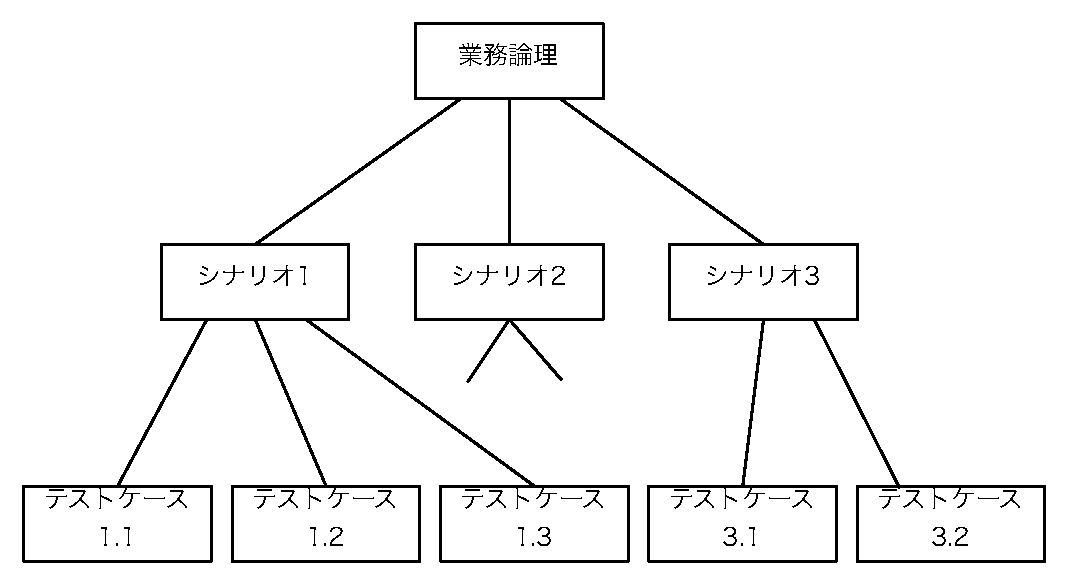
\includegraphics[width=55zw, keepaspectratio]{./Chapter4/image/SpecTree.pdf}}
	\caption{業務論理とシナリオとテストケースの対応関係}
	\label{fig:SpecTree}
	\index{ぎょうむろんりとてすとけーすのたいおうかんけい@業務論理とシナリオとテストケースの対応関係}
\end{figure}


	要求辞書階層は、業務論理階層で使う用語を定義している。
		\index{ようきゅうじしょかいそう@要求辞書階層}
	この階層では、名詞に対応するクラス名や型名だけでなく、
	動詞に対応する関数(function)や操作(operation)も記述する。
	この階層に記述される仕様は、いわゆる暗黙知の明示的な仕様となるため、
		\index{あんもくち@暗黙知}
	何を記述すべきかも含めて、記述は容易ではないが、この階層が記述できることにより、
	暗黙知を明示的な知識として共有することができるようになる。
	したがって、要求辞書階層の再利用性は、同じ問題領域であれば、かなり高い。
	要求辞書階層を記述する仕様記述者は、VDM++の構文をある程度マスターしていなければならない。

	\ref{FareModel}章で紹介する運賃計算モデルの仕様記述フレームワークを、表\ref{SpecFrameFare}に示す。

\begin{table}[h]
	\caption[仕様記述フレームワーク(フェリカネットワークス)]{仕様記述フレームワーク(運賃計算モデル)}
	\index{しようふれーむわーくうんちんけいさんもでる@仕様記述フレームワーク(運賃計算モデル)}
	\label{SpecFrameFare}
	\begin{center}
		\setlength{\tabcolsep}{3pt}
		\begin{tabular}{|l|l|l|} \hline
			仕様記述の階層 & 充足する記述領域 & 必要なVDM技量  \\ \hline\hline
			テストケース  & 回帰テスト & 初級 \\ \hline
			業務論理  & 業務アプリケーション & 初級 \\ \hline
			要求辞書  & 業務知識兼用語辞書 & 中級 \\ \hline
			ユーティリティ  & 共通機能 & 上級 \\ \hline
		\end{tabular}
	\end{center}
\end{table}

	この運賃モデルは、教育用に基本的な機能だけを持った仕様を記述しているため、
	仕様記述フレームワークの階層も深くはない。

	ユーティリティ階層は、鉄道ネットワークのグラフ構造から最短距離を計算する
	ダイクストラ算法のために作った。
	当然ながら、ユーティリティ階層の再利用性は、要求辞書階層よりも更に高い。

	図\ref{fig:ClassDiagram4Fare}に、
	運賃計算モデルのクラス図と、仕様記述フレームワーク階層の対応関係を示す。

\begin{figure}[h]
	\centering
	{\includegraphics[width=55zw, keepaspectratio]{./Fare/image/ClassDiagram.jpg}}
	\caption{運賃計算モデルのクラス図}
	\label{fig:ClassDiagram4Fare}
	\index{うんちんけいさんもでるのくらすず@運賃計算モデルのクラス図}
\end{figure}

	仕様記述フレームワークの各階層の具体例については、\ref{FareModel}章を参照していただきたい。

\subsection{仕様ライブラリ}
	\label{SpecLibrary}
	\index{しようらいぶらり@仕様ライブラリ}

	以下のライブラリ3000行ほどを、あらかじめ作成した。

	\begin{itemize}
	\item 文字、文字列ライブラリ \\
		VDM++は、特定の文字コードに依存しないよう、文字、文字列順という概念がないが、
		エンタープライズ系のシステムではソート順として多用されるため。
	\item 暦、日時、期間ライブラリ \\
		エンタープライズ系のシステムでは、暦、日時、期間などに関する欠陥が多いため。
	\item 列ライブラリ \\
		エンタープライズ系のシステムでは、合計、平均、ソートなどが多用されるため。
	\item 待ち行列、ハッシュ表ライブラリ \\
		データ構造としてよく使われるため。
	\item 数値計算関連ライブラリ \\
		実数の桁数、微分、ニュートン法などを使うことが予想されたため。
	\item その他、業務に関連したライブラリ
	\end{itemize}

\section{仕様テスト}
	\label{SpecTest}
	\index{しようてすと@仕様テスト}

	仕様のテストは、以下のようにして行った
	\footnote{詳細については、VDMTools ユーザマニュアル(VDM++) 2.0
		{\url{http://www.vdmtools.jp/modules/tinyd2/index.php?id=2}}
	を参照のこと}
	。

	\begin{itemize}
	\item VDMToolsで、静的チェック
		\begin{itemize}
		\item 構文チェック、型チェック \\
			\index{こうぶんちぇっく@構文チェック}
			\index{かたちぇっく@型チェック}
			型チェックは、当初予想していたより、はるかに多くの単純ミスを発見した。
		\item 証明課題生成を行ってレビュー \\
			\index{しょうめいかだいせいせい@証明課題生成}
			事前条件の記述忘れを、かなりの確率で発見できた。
		\end{itemize} 
	\item VDMToolsで、動的チェック \\
		\index{どうてきちぇっく@動的チェック}
		VDM++インタープリタとデバッガで実行可能仕様
		\index{じっこうかのうしよう@実行可能仕様}
		\footnote{陽仕様とも言う}
		をテストした。
		\begin{itemize}
		\item 動的に、不変条件・事前条件・事後条件をチェック
			\index{ふへんじょうけん@不変条件}\index{じぜんじょうけん@事前条件}\index{じごじょうけん@事後条件}
		\item 組合せテスト機能を利用して、組合せテスト(\ref{CombinatorialTest}参照)を実行
			\index{くみあわせきのう@組合せテスト機能}
		\item 回帰テスト支援ライブラリを改良して回帰テスト(\ref{RegressionTest}参照)を実行 \\
				\index{かいきてすと@回帰テスト}
				回帰テストケースを作成するのはそれなりに大変だが、仕様修正に対して非常に効果があった。
		\item コードカバレージ(網羅性検査)機能で、テスト達成率を測定 \\
				\index{こーどかばれーじ@コードカバレージ}\index{もうらせいけんさ@網羅性検査}
				C0(命令)レベルで、
				85\%(フェリカネットワークス事例(\ref{FeliCa}節))から95\%(日本フィッツ事例(\ref{JFITS}節))を達成した。
		\item 検出した矛盾点を、要求仕様に反映
		\end{itemize} 
	\item VDM仕様に基づいて、ランダム評価ツールを作成し、
			数億件のテストケースを生成し、動的チェック(フェリカネットワークス事例)を行った。
		\begin{itemize}
		\item 仕様エミュレータを内蔵
		\item 実装に対し、ランダムにコマンドを送信し、応答が正しいか確認
		\end{itemize} 
	\end{itemize} 

\subsection{組合せテスト}
	\label{CombinatorialTest}
	\index{くみあわせてすと@組合せテスト}

	組合せテスト(Combinatorial Test)は、指定したテストパターンから、テストケースの組合せを生成し、テストする。
	テストでエラーになったものと同じパターンのテストケースは実行せず、テストの実行効率を上げる。

	下記の例のように、trace句の後に組合せテストケースを記述する。
	各組合せテストケースはラベル(今の場合S1, S2など)で始まり、
	VDMの構文の後ろに組合せの正規表現記述を行う。
		\index{せいきひょうげんきじゅつ@正規表現記述}
	正規表現記述の説明は、VDM++の注釈として示した。

\begin{verbatim}
class UseUniqueNumber
instance variables
sUN : 発番者 :=  new 発番者();

traces
S1 :  let n in set {1,2,3,4} in sUN.発番する(n){10,12}   -- 10回から12回繰り返す

S2 :  let n in set {2} in sUN.発番する(n)+   -- 1回から既定回数繰り返す

S3 :  let n in set {3} in sUN.発番する(n)*   -- 0回から既定回数繰り返す

S4 :  let n in set {4} in sUN.発番する(n){10002}   --10002回繰り返す

end UseUniqueNumber
\end{verbatim}

図\ref{fig:CombinatorialTestScreen}に、組合せテスト実行後のOverture tool画面例を示す
\footnote{VDMToolsは、組合せテスト実行結果をインタープリタ・ウィンドウにログとして表示する}。

\begin{figure}[h]
	\centering
	{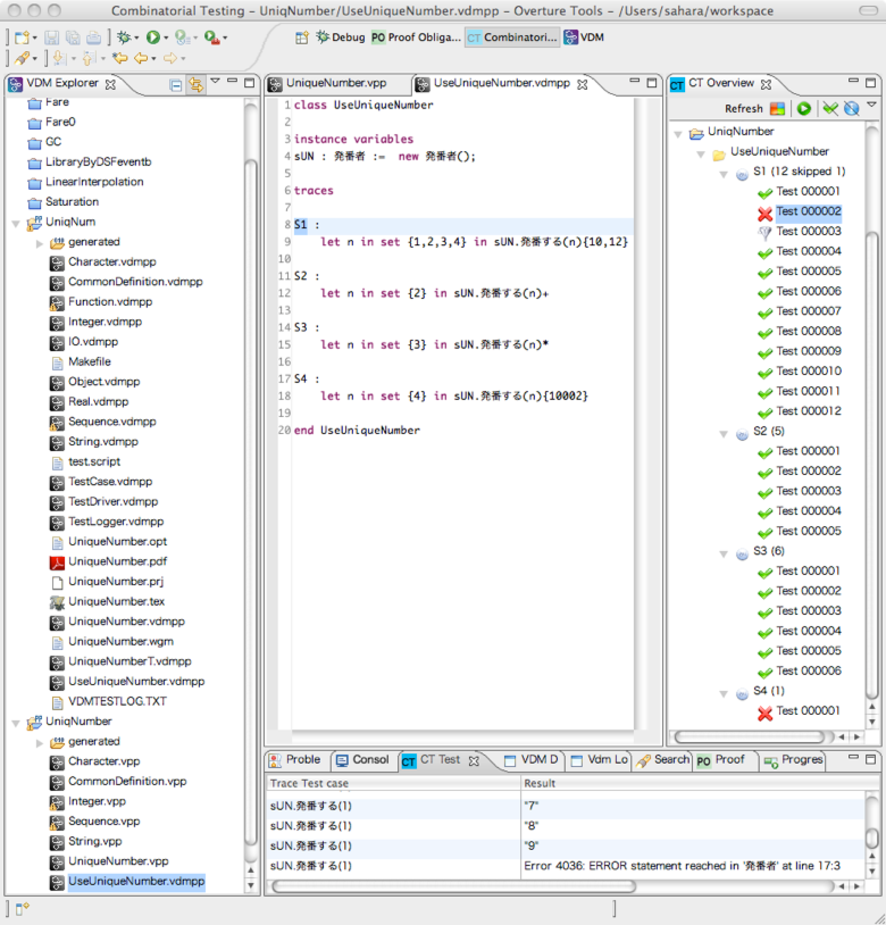
\includegraphics[width=55zw, keepaspectratio]{./UniqNumber/image/CombinatorialTestScreen.pdf}}
	\caption{組合せテスト実行画面例}
	\label{fig:CombinatorialTestScreen}
	\index{くみあわせてすとじっこうがめんれい@組合せテスト実行画面例}
\end{figure}

図\ref{fig:CombinatorialTestScreen}右上のCT Overviewサブ・ウィンドウに組合せテストの実行結果が表示されている。

テストS1の最初のテストTest 000001は正常終了したので、緑色のチェックマークが付く。
もちろん、正常終了したからといって、このテストケースが正しいとは限らない。
不変条件、事前条件、事後条件が正しく記述されている場合は意味的にも正しいが、
それ以外の場合は、単に実行が正常に終了したことを示すだけであって、
意図した結果が得られているとは限らないので、注意が必要である。

次の、Test 000002は実行時エラーがあったことを示して、赤色の×マークが付いている。
このエラー原因は、右下のCT Testサブ・ウィンドウに示されていて、
発番者クラス17行目第3カラムでERROR文が実行されたことが示されている。
ERROR文は、エラーがあったことを示して停止するだけなので、
エラー原因は発番者クラスのVDM++ソースを見て判断しなければならない
\footnote{エラー原因を表示するようにVDM++仕様を作成することは、例外処理文などを使えば可能である。
ここでは、説明の単純化のためにERROR文を使った}。

Test 000003は、Test 000002と同じ順序でテストケースを実行するため、
必ず同じ所でエラーとなるので、それを検知した組合せテストケース機能が、
実行せずにエラーを表示している。この印が漏斗のような灰色のアイコンである。

組合せテストは、このようにして、数千件のテストケースを実行できるので、
複雑な組合せ条件をテストするのに適している。


\subsection{回帰テスト}
	\label{RegressionTest}
	\index{かいきてすと@回帰テスト}

	回帰テスト(regression test)は、ソフトウェアが退化していないか確認するテストである。
	テストケースと期待する結果を一体にして記述し、実行して一致するか確認する。

	VDM++では、VDMUnitと呼ばれる回帰テスト用ライブラリを使用して回帰テストを行う。

	回帰テスト実行用のクラスは\ref{RegressionTestExecute}節のTestAppクラスを参照していただきたい。
	回帰テストケースは、\ref{RegressionTestcase}節の回帰テストケースクラスと、そのサブクラス群を参照していただきたい。

	回帰テストのノーマルケースの例は、\ref{RegressionTestNormalCase}節のTestCaseT0001クラスを参照のこと。
	回帰テストのエラーケースの例は、\ref{RegressionTestErrorCase}節のTestCaseT0003クラスを参照のこと。


\section{プログラミング}
	\label{Programming}
	\index{ぷろぐらみんぐ@プログラミング}

	VDM++仕様を見ながら、以下の作業を行った。

	\begin{itemize}
	\item 実装用フレームワークを作成
	\item VDM++仕様を見て、手作業でプログラム作成 \\
		VDM++からC++生成も可能だが
		\begin{itemize}
		\item 独自のミドルウェアに合わせて調整する時間的余裕が無かった(日本フィッツ事例)。 \\
					生成されるプログラムの性能は、恐らく問題ないと予想したが
						\footnote{SCSKでは、現在、コード生成機能を大幅に改良し、
							エンタープライズシステム用Java生成フレームワークを試作中。}、
					プロジェクト工数の5\%程度の作業に時間を取られたくなかったため、
					プログラム生成は使用しなかった。
		\item 生成されたC++プログラムの性能が、十分でなかった(フェリカネットワークス事例)。
		\end{itemize} 
	\item 単純な画面生成プログラムを作成し、GUI生成(日本フィッツ事例)。
	\item オランダの花市場オークションシステム事例では
		\index{おらんだのはなしじょうオークションしすてむ@オランダの花市場オークションシステム事例}
		1999年にC++生成を利用し、ソースの90\%を生成。残りは、手でコーディング。
	\end{itemize} 

\section{プログラムのテスト}
	\label{TestOfProgram}
	\index{ぷろぐらむのてすと@プログラムのテスト}

	プログラムのテストは以下のように行った。

	\begin{itemize}
	\item 単体テスト
		\index{たんたいてすと@単体テスト}
		\begin{itemize}
		\item Purify
				\footnote{現在の製品名は、Rational PurifyPlus。
					\url{http://www-06.ibm.com/software/jp/rational/products/purifyp/highlights.html}}
				でソースの静的チェック \\
				メモリの破壊可能性などをチェックした。
		\item C++コードカバレージ機能でテスト達成率測定
			\begin{itemize}
			\item Excelデータからテストケースを生成する簡単なプログラムを作成 \\
				メモリの破壊可能性などをチェックした。
			\item VDM++テストケースを、C++プログラムのExcelの単体テストケースに手作業で変換 \\
				C0レベルで98\%カバー
			\end{itemize} 
		\item 仕様エミュレータを内蔵(フェリカネットワークス事例) \\
				実装に対し、ランダムにコマンドを送信し、応答が正しいか確認(フェリカネットワークス事例)
		\end{itemize} 
	\item 連結テスト \\
		要求定義担当者が、業務知識とWordで作成したユースケースから、テストケース生成(日本フィッツ事例)
	\item 総合テスト
		\index{そうごうてすと@総合テスト}
		\begin{itemize}
		\item 評価環境を構築(フェリカネットワークス事例) \\
			ICチップファームウェアと、実装と、形式仕様とが、同様の動作をすることを確認。
		\item VDM仕様に基づいて、ランダム評価ツールを作成し、数億件のテストケースを生成し、
			動的チェック(フェリカネットワークス事例)
		\item 業務専門家全員で総合テストケース作成 (日本フィッツ事例)
		\end{itemize} 
	\end{itemize} 

\section{開発管理}
	\label{DevelopmentManagement}
	\index{かいはつかんり@開発管理}

	開発管理は、開発時点で実用性があると分かっていたソフトウェア工学技術とツールを使用して、
	以下のように行った。

	\begin{itemize}
	\item 版管理ツールcvsを使用 \\
			\index{はんかんりつーる@版管理ツール}
			VDM++仕様、ソースプログラム、Wordなどのドキュメント、テストケース、
			プログラム実行モジュールなど、全てのリソースを版管理した。
	\item Swiki(Squeak Wiki)サーバーを使って、共同作業を円滑にした(日本フィッツ事例)。
	\item ISO\,9000にしたがって、単体テスト以後の全欠陥をnotesで記録し、追跡した (日本フィッツ事例)。
	\end{itemize} 

\section{開発体制}
	\label{DevelopmentTeamStructure}
	\index{かいはつたいせい@開発体制}

\subsection{日本フィッツの開発体制}
	\index{にほんふぃっつのかいはつたいせい@日本フィッツの開発体制}

	仕様作成チーム、実装チーム、証券業務専門家チームの間で、相互チェックを行いながら開発を行った。

	証券業務専門家チームは、ユースケースの最初の案をWordで作成し、VDM++仕様の回帰テスト結果を主としてチェックした。
	VDM++ソースのチェックは、計算式部分など一部のみ行った。
	テスト工程では、連結テスト、総合テストのテストケース作成と結果の確認を行った。

	仕様作成チームは、Wordで記述されたユースケース相当の仕様をチェックしながら、
	VDM++では、ほぼ完全にそれらを書き換えた。
	プログラムの単体テスト工程では、実装チームの作成したテストケースとVDM++仕様のテストケースを目で比較し、
	不足しているテストケースを追加した。

	実装チームは、VDM++仕様を全て読み、手作業でプログラムに変換した。
	他チームの成果物のほとんどをレビューし、チェックした。
	

\subsection{フェリカネットワークスの開発体制}
	\index{ふぇりかねっとわーくすのかいはつたいせい@フェリカネットワークスの開発体制}

	仕様作成チーム、評価チーム、実装チームの間で、相互チェックを行いながら開発を行った。

	各チームの相互チェックの様子を、図\ref{fig:FeliCaTeamStructure}に示す。

\begin{figure}[h]
	\centering
	{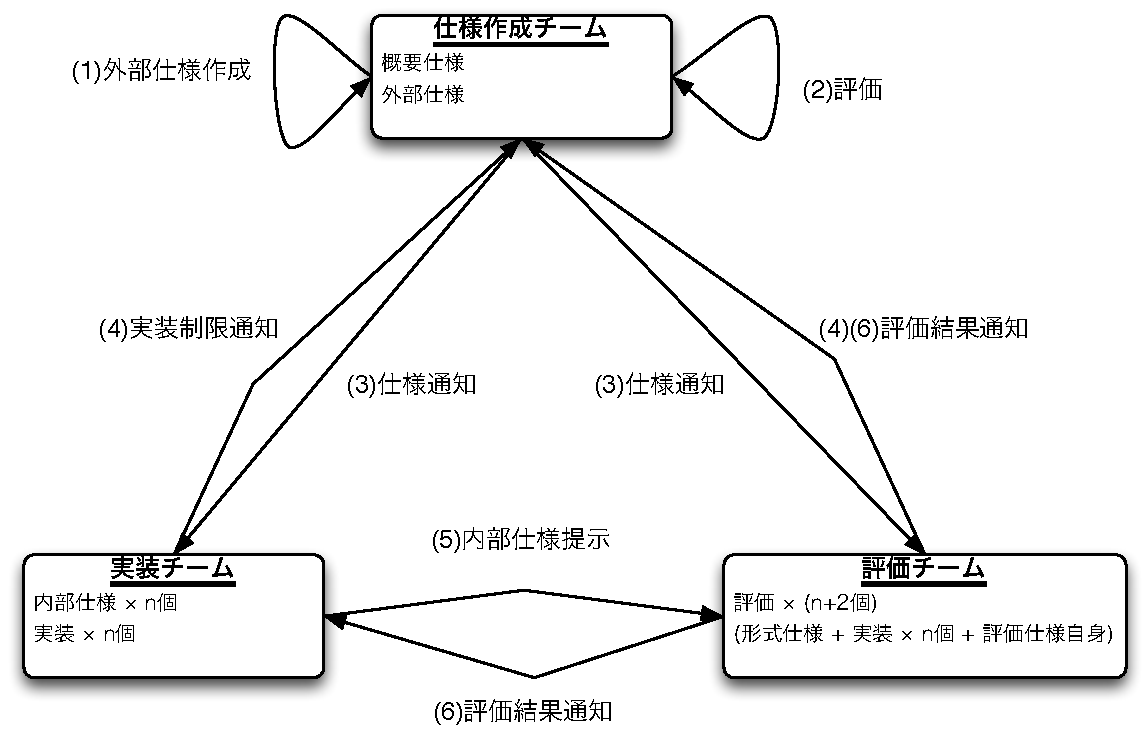
\includegraphics[width=55zw, keepaspectratio]{./Chapter4/image/FeliCaTeam.pdf}}
	\caption{フェリカネットワークスの開発体制}
	\label{fig:FeliCaTeamStructure}
	\index{ふぇりかねっとわーくすのかいはつたいせい@フェリカネットワークスの開発体制}
\end{figure}

\begin{enumerate}
	\item 仕様作成チームは、日本語の概要仕様からVDM++による外部仕様を作成し、
	\item 回帰テストを行って、外部仕様の評価(正当性検証と仕様作成チームの観点からの妥当性確認)を行い、
	\item 評価チームと実装チームに評価済みの仕様を通知する。
	\item 評価チームは、評価チームの評価結果を仕様作成チームにフィードバックし、\\
		実装チームは、内部仕様と実装を通して発見した、実装上の制限を仕様作成チームにフィードバックする。
	\item 実装チームは、作成した内部仕様を評価チームに提示し、
	\item 評価チームは、VDM++による形式仕様と、n個のチップの実装仕様と、評価仕様自身を総合して評価し、\\
		実装チームおよび仕様作成チームに評価結果をフィードバックする。
\end{enumerate}

	

\chapter {対象を如何にモデル化するか?}
	\label{How2MakeModel}
	対象を如何にモデル化するかということは、
こうやれば誰でも確実に良いモデルができるという一般的手順があるわけではない。
しかし、数学やソフトウェア工学の歴史の中で培われた一般的原則と手順はある。
本章では、このような一般的原則と手順を紹介する。
何らかの仕様記述言語を前提としないと説明が難しいので、VDM++言語を前提とする。

これらの原則と手順は、
構造化分析・設計手法(SA/SD)やオブジェクト指向分析・設計手法(OOA/OOD)におけるモデル化手法と、
より品質を高める形式手法の技術を除けば、さほど違いがあるわけではない。
	\index{こうぞうかぶんせきせっけいしゅほう@構造化分析・設計手法(SA/SD)}
	\index{おぶじぇくとしこうぶんせきせっけいしゅほう@オブジェクト指向分析・設計手法(OOA/OOD)}

\section {モデル化の一般的手順}
\index{もでるかのいっぱんてきてじゅん@モデル化の一般手順}

\begin{enumerate}
\item モデル化の範囲を決める。
	\index{もでるかのはんいをきめる@モデル化の範囲を決める}

	例えば、「エラー処理の詳細を除くユースケースレベルの要求仕様を書く」とか、
	「アプリケーションレベルのエラー処理の詳細も含めて、外部仕様相当の設計仕様を記述する」といった方針を決める。
	過去に成功した形式手法使用プロジェクトの調査結果\cite{SEC2012FMREPORT}では、この範囲決めが重要で、
	かつ、この範囲内をすべて形式仕様で記述することが形式手法採用プロジェクト成功の鍵であることが分かっている。

\item 仕様を分割統治する。
	\index{しようをぶんかつとうちする@仕様を分割統治する}

	階層化とモジュール化(\ref{SpecFramework}節と\ref{sec:specFM}節で紹介する仕様記述フレームワークを使う)を行い、
	ある階層やモジュールの変更余波が、他の階層やモジュールに及ばないようにモデルを構築する。

	これによって、モデルの保守性や再利用性が増し、可読性も増す。

\item 主に名詞から型を定義する。
	\index{めいしからかたをていぎする@名詞から型を定義する}

	属性の参照に留まらない機能を持つ型は、クラスとする。

\item システムが状態を持つ場合、その状態を定義する。
	\index{じょうたいをていぎする@状態を定義する}

	VDM++の場合、状態はインスタンス変数として持つ。

\item 主に、述語(動詞)から、関数・操作のインタフェース(シグネチャという)を記述する。
	\index{じゅつごからかんすうそうさのいんたふぇーすをていぎする@述語から、関数・操作のインタフェースを記述する}

\item 関数・操作の事後条件・事前条件を記述する(陰仕様
		\footnote{関数・操作のインタフェースと、事前条件及び事後条件しか記述していない仕様を陰仕様と呼ぶ。
		陰仕様は、関数・操作の本体は記述していないが、「仕様」を記述していることになる。}
	作成)。
	\index{いんしようをさくせいする@陰仕様を作成する}

	事後条件は、関数ないし操作が終わった状態を真(true)を返す論理式で表す。
	したがって、関数ないし操作の「仕様」と言える。

	事前条件は、引数の制約条件を論理式で記述し、仕様の責任を明確化するためのものである。
	すなわち、事前条件が偽となる引数に対して責任を負わないことを宣言している。
	操作の場合は、インスタンス変数の制約条件も記述することができる。

\item 静的検証を行う。
	\index{せいてきけんしょうをおこなう@静的検証を行う}

	構文・型・証明課題チェックをツールを使用して行う。
	この段階で、多くの単純ミスが検出され、仕様作成者は「仕様の意味」に集中することができる。
	

\item 関数・操作の本体を記述する(陽仕様
		\footnote{関数・操作の本体が記述されていて実行可能な仕様を陽仕様と呼ぶ。}
	にする)。
	\index{ようしようをさくせいする@陽仕様を作成する}

	陰仕様は、静的検証以外の検証ができないため、事後条件を満たすか否かの動的検証を行うために、
	関数・操作の本体を記述する。

	事後条件を満たす本体の記述は幾通りもあり得るし、本体の記述は一つの実装を表しているので、
	本体は、仕様そのものではなく、事後条件で記述された「仕様」が正しいことを検証するためのものである、と言える。
	

\item モデルの正当性と妥当性を、動的に検証・確認する。
	\index{もでるのせいとうせいとだとうせいをどうてきにけんしょうかくにんする@モデルの正当性と妥当性を動的に検証・確認する}

	ツールのインタープリタ、デバッガを使用して、モデルの正当性(verification)を検証し妥当性(validation)を確認する。

\item 要求仕様をレビューし、漏れがないか再検討する。
	\index{ようきゅうしようをれびゅーする@要求仕様をレビュー}

	形式手法を使っていても、仕様作成者やユーザーによるレビューは必要である。
	意味的な仕様の整合性は、人間しか気が付かない事が多いからである。
\end{enumerate}
	本章では、対象を如何にしてモデル化するかを、鉄道会社Aの特急券予約システムを例にして説明する。
これは、乗客として特急券予約システムを使う際に起きたトラブルの原因を追求するために作成したモデルである。

\section {特急券予約システムの例}
	\index{えくすぷれすよやくのれい@特急券予約システムの例}

\subsection{問題点の要約}
	\addcontentsline{toc}{section}{問題点の要約}
	\index{もんだいてんのようやく@問題点の要約}

問題の発端は、クレジットカード会社の都合で、
特急券予約システムに使用していたクレジットカードを変更せざるを得なくなり、
特急券予約システムの設定を変更しようとしたところから始まった。

\begin{enumerate}
\item 客(すなわち筆者)は、おサイフケータイ(鉄道会社B)で特急券予約システム(鉄道会社A)を使っていた。
\item 会社Cクレジットカードが廃止になり会社Dクレジットカードに変更して下さいとの連絡があった。
\item 鉄道会社Aサポートセンターに電話したところ、
	おサイフケータイの登録クレジットカードを変更すれば、2日後には特急券予約システムが使えますとのことだった。
\item おサイフケータイの設定でクレジットカードを変更し、2日後に使おうとしたが、特急券の予約ができなかった。
\item 予約できなかったので 鉄道会社Aサポートセンターに電話

	\begin{description}
	\item [客]「特急券を2枚予約しようとしたが、予約できなかったんですが?」
	\item [鉄道会社A]「カードを変更したら、新規に特急券予約システムを契約して下さい。」
	\item [客]「新規にすると会費がかかるのでは?」
	\item [鉄道会社A]「はい。」
	\item [客]「カード会社の都合で変更するのに、それはおかしいでしょう?」
	\item [鉄道会社A]「では、無料にします。」
	\end{description}

\item 特急券に引き換えできなかったので 鉄道会社Aサポートセンターに電話

	\begin{description}
	\item [客]「新しい予約はできたんですが、クレジットカード変更前に予約した特急券に引き換えようとしたらできないのですが?」
	\item [鉄道会社A]「予約会員証で引換できるようになったので、それで引き換えて下さい。
			暗証番号はクレジットカードのものを使って下さい。」
	\end{description}

\item T駅での問答

	\begin{description}
	\item [客]「会員証で特急券に引き換えできないのですが?」
	\item [鉄道会社A]「会員証で引き換えできないですねー。おかしいな。クレジットカードでやってみましょう。駄目ですねー。」
	\item [客]「古いクレジットカードでは駄目ですか?」
	\item [鉄道会社A]「あ、できましたね。はい、切符です。」
	\end{description}

\end{enumerate}

\subsection {モデル化対象用語の選択}
	\addcontentsline{toc}{section}{モデル化対象用語の選}
	\index{もでるかたいしょうようごのせんたく@モデル化対象用語の選択}


前節のやりとりは、電話でのやりとりをかなり(主として用語を中心として)整理したものである。
実際には、例えば、鉄道会社Aサポートセンターの担当者は「カード」という言い方をするのだが、
それがクレジットカードの場合と、予約会員証の場合と、
IC カードあるいは予約カードの場合があったので、
個々の用語の正確な名前と意味を調べるだけで
かなりの日数と時間を要した問答であった。

この問題で登場する用語は、インターネットなどで調べたところ以下に示すものががあった。

\begin{itemize}
\item 鉄道会社A、鉄道会社B
\item おサイフケータイ
\item 特急券予約システム
\item 予約会員証、ICカード、予約カード
\item クレジットカード
	\begin{itemize}
	\item 会社Cクレジットカード、会社Dクレジットカード
	\end{itemize} 
\item 特急券
\end{itemize} 

ICカードと予約カードは、結局、この問題とは直接は関係なかったので、
モデルを単純化するため対象としないことにした。

「鉄道会社B」をモデル化すると、さらに問題点が見つかるとは思ったが、
今回の「特急券に引き換えできない問題」の解決には直接関係ないと思ったので、
モデルを単純化するため対象としなかった。

このように、モデルを単純化し、一番問題となりそうなところからモデル化を始め、
検証して問題がないことを確認し、
必要があればモデルを拡張していくのがモデル化のコツである。

\subsection {モデル化する機能の範囲選択}
	\addcontentsline{toc}{section}{モデル化する機能の範囲選択}
	\index{もでるかするきのうのはんいせんたく@モデル化する機能の範囲選択}


「鉄道会社A」の「特急券予約システム」のうち、
今回の問題に直接関係する
以下の機能だけをVDM++\cite{SCSK2012PP}で要求仕様としてモデル化し、
問題点を明確化することにした。
\footnote{仕様記述言語としてVDM++を採用したのは、
開発現場に導入するのが最も容易な形式仕様記述言語と判断したからである。
}

\begin{itemize}
\item 予約する
\item 特急券を得る
\item クレジットカードを切り替える
\end{itemize} 

したがって、モデル化する範囲に登場する主要な用語は以下だけである。
\begin{itemize}
\item おサイフケータイ
\item 特急券予約システム
\item 特急券予約
\item 予約会員証
\item クレジットカード
\item 特急券
\end{itemize} 

この用語と先程モデル化することにした機能を表す文(「予約する」、「特急券を得る」など)を併せて辞書とし、
要求辞書と呼ぶこともある。
	\index{ようきゅうじしょ@要求辞書}

\subsection {仕様記述フレームワークの設定}
	\addcontentsline{toc}{section}{仕様記述フレームワークの設定}
	\index{しようきじゅつふれーむわーくのせってい@仕様記述フレームワークの設定}
	\label{sec:specFM}

仕様を作成する際、仕様作成者各自が独自の形式で作成すると、
保守性や再利用性に悪影響が出る。
	\index{ほしゅせい@保守性}\index{さいりようせい@再利用性}

そこで、仕様を階層分けしてカプセル化し、
	\index{かぷせるか@カプセル化}
各階層で充足すべき記述領域を明確化して、保守性と再利用性の向上を図った。

このような仕様記述フレームワークを作っておくと、
各階層毎の記述に必要なVDM++言語の知識も局所化でき、
全員がVDM++に精通していなくても、仕様記述が可能になることが、
経験上分かっている。

本モデルの記述に際して使用する仕様記述フレームワークの階層は、表\ref{SpecLevel1}のようになる。

\begin{table}[h]
	\caption[仕様の階層(特急券予約システム)]{仕様の階層(特急券予約システム)}
	\index{しようのかいそうとっきゅうけんよやくしすてむ@仕様の階層(特急券予約システム)}
	\label{SpecLevel1}
	\begin{center}
		\setlength{\tabcolsep}{3pt}
		\begin{tabular}{|l|l|l|l|} \hline
			仕様記述の階層 & 充足する記述領域 & 備考 & 必要なVDM技量  \\ \hline\hline
			テスト & 回帰テスト & & 初級 \\ \hline
			業務論理 & 業務アプリケーション &  構造化日本語仕様 & 初級\\ \hline
			要求辞書 & 業務知識兼用語辞書 & ドメイン・オブジェクトも含まれる & 中級 \\ \hline
			ユーティリティ & 共通機能 & & 上級〜中級 \\ \hline
		\end{tabular}
	\end{center}
\end{table}

表\ref{SpecLevel1}で、業務論理階層の記述は、
業務アプリケーションを記述する日本語識別子を使った構造化日本語仕様と見なすこともできる。

日本語で擬似コードを使った仕様を書くことがあるが、
この場合は逆に、厳密で明確な文法を持ったVDM++の仕様を日本語による擬似コードのように読めるよう工夫することで、
読みやすさと厳密な記述による品質向上の両方を目指そうという訳である。


\subsection {VDM++モデル例}	
	\addcontentsline{toc}{section}{VDM++モデル例}
	\index{VDM++モデルれい@VDM++モデル例}
	\label{VDMModelExpressReservation}

以下に、特急券予約システムをVDM++で記述したモデルを示す。
	\index{とっきゅうけんよやくしすてむをVDM++できじゅつしたもでる@特急券予約システムをVDM++で記述したモデル}

このモデルは、要求仕様記述レベルであるが、
アプリケーションレベルのエラー処理は記述せず、
不変条件と事前条件および事後条件の記述を行う。
すなわち、要求仕様記述・分析工程で最初に記述し検証する、
最も抽象的なモデルである。
	\index{ちゅうしょうてきなもでる@抽象的なモデル}

要求仕様記述・分析工程の最後では、
アプリケーションレベルのエラー処理をすべて記述する、
詳細な要求仕様を記述するが、
	\index{しょうさいなようきゅうしよう@詳細な要求仕様}
通常、その規模は最初の抽象的な要求仕様より10倍ほどになるので、
本ブックレットでは紹介できなかった。

静的検証と動的検証の両方を使って正当性検証と妥当性確認を行う。
動的検証は、仕様アニメーション、すなわち仕様実行によって行う。

特急券予約システムの、主要なクラスを記述したクラス図は図\ref{fig:ExpressReservationClassDiagram}のようになった。
このクラス図は、最初からこのような形をしていたわけではなく、
VDM++でモデル化をしつつ、検証しながら、徐々に整理してこのような形となった。
\footnote{
このクラス図は、VDMToolsから生成し、astah professionalによって整形したものである。
}

\begin{figure}[h]
	\centering
	{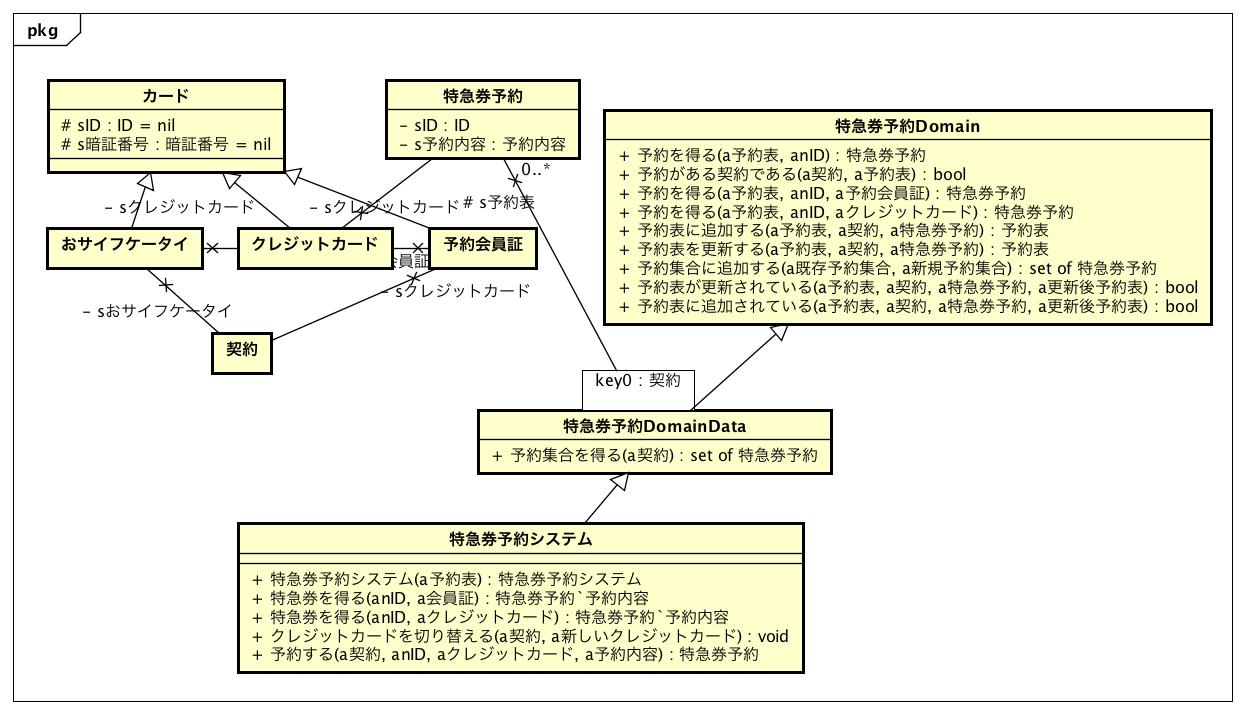
\includegraphics[width=55zw, keepaspectratio]{./ExpressReservation/image/ClassDiagram.jpg}}
	\caption{クラス図(特急券予約システム)}
	\label{fig:ExpressReservationClassDiagram}
	\index{くらすすとっきゅうけんよやくしすてむ@クラス図(特急券予約システム)}
\end{figure}

各クラスと、仕様階層の対応は、表\ref{SpecLevel2}のようになる。

\begin{table}[h]
	\caption[特急券予約システムの仕様の階層]{特急券予約システムの仕様の階層}
	\index{えくすぷれすよやくのしようのかいそう@特急券予約システムの仕様の階層}
	\label{SpecLevel2}
	\begin{center}
		\setlength{\tabcolsep}{3pt}
		\begin{tabular}{|c|l|} \hline
			階層 & クラス   \\ \hline\hline
			テスト & TestApp \\ \cline {2-2}
			  & 回帰テストケースクラス(TestCaseT0001など) \\ \hline
			業務論理 & 特急券予約システム \\ \hline
			要求辞書 & 特急券予約システムDomain   \\ \cline {2-2}
			  & 特急券予約システムDomainData \\ \cline {2-2}
			  & 契約   \\ \cline {2-2}
			  & 特急券予約システム  \\ \cline {2-2}
			  & クレジットカード  \\ \cline {2-2}
			  & 予約会員証  \\ \cline {2-2}
			  & おサイフケータイ \\ \hline
			ユーティリティ & 回帰テストユーティリティなど \\ \hline
		\end{tabular}
	\end{center}
\end{table}

	
%\section {発端}
鉄道会社Aの特急券予約システムで特急券を2枚予約し、
以下のような「事件」が起こったのが本モデルを書いた理由である。


以下のやりとりは、電話でのやりとりをかなり(主として用語を中心として)整理したものである。
実際には、例えば、鉄道会社Aサポートセンターの担当者は「カード」という言い方をするのだが、
それがクレジットカードの場合と、予約会員証の場合と、ICカードあるいは予約カードの場合があったので、
個々の用語の正確な名前と意味を調べるだけで
かなりの日数と時間を要した問答であった。

ICカードと予約カードは、結局、この問題とは直接は関係なかったので、この後、本稿に登場することはない。

\begin{itemize}
\item おサイフケータイ(鉄道会社B)で特急券予約システム(鉄道会社A)を使っていた
\item ロンロンViewカードが廃止になりアトレクラブViewカードに変更して下さいとの連絡があった
\item 予約できなかったので 鉄道会社Aサポートセンターに電話

	\begin{description}
	\item [客]「特急券を2枚予約しようとしたが、予約できなかったんですが?」
	\item [JR]「カードを変更したら、特急券予約システムを新規に契約して下さい。」
	\item [客]「新規にすると会費がかかるのでは?」
	\item [JR]「はい。」
	\item [客]「カード会社の都合で変更するのに、それはおかしいでしょう?」
	\item [JR]「では、無料にします。」
	\end{description}

\item 特急券に引換えできなかったので 鉄道会社Aサポートセンターに電話

	\begin{description}
	\item [客]「新しい予約はできたんですが、クレジットカード変更前に予約した特急券に引換えようとしたらできないのですが?」
	\item [JR]「予約会員証で引換できるようになったので、それで引換えて下さい。
			暗証番号はクレジットカードのものを使って下さい。」
	\end{description}

\item T駅での問答

	\begin{description}
	\item [客]「会員証で特急券に引換えできないのですが?」
	\item [JR]「会員証で引換えできないですねー。おかしいな。クレジットカードでやってみましょう。駄目ですねー。」
	\item [客]「古いクレジットカードでは駄目ですか?」
	\item [JR]「あ、できましたね。はい、切符です。」
	\end{description}

\end{itemize} 


\section {モデル化の範囲}
この問題で登場する用語には以下がある。

\begin{itemize}
\item 鉄道会社A、鉄道会社B
\item おサイフケータイ
\item 特急券予約システム
\item 予約会員証、ICカード、予約カード
\item クレジットカード
	\begin{itemize}
	\item ロンロンViewカード、アトレクラブViewカード
	\end{itemize} 
\item 特急券
\end{itemize} 

「鉄道会社B」「ICカード」「予約カード」は、モデルを単純化するため対象としなかった。

「鉄道会社A」の「特急券予約システム」システムのうち、
以下の機能だけをVDM++\cite{SCSK2012PP}で要求仕様としてモデル化し、
問題点を明確化することにした。

\begin{itemize}
\item 予約する
\item 特急券を得る
\item クレジットカードを切り替える
\end{itemize} 

従って、モデル化する範囲に登場するpublicな用語は以下だけである。
\begin{itemize}
\item おサイフケータイ
\item 特急券予約システムシステム
\item 特急券予約システム
\item 予約会員証
\item クレジットカード
\item 特急券
\end{itemize} 





	
	\include{ExpressReservation/ReservationSysytem.vpp}	
	\include{ExpressReservation/Common.vpp}
	\include{ExpressReservation/ReservationDomain.vpp}
	\include{ExpressReservation/ReservationDomainData.vpp}
	\include{ExpressReservation/ExpressReservatiopn.vpp}
	\include{ExpressReservation/Contract.vpp}
	\include{ExpressReservation/Card.vpp}
	\include{ExpressReservation/CredirCard.vpp}
	\include{ExpressReservation/CustomerCard.vpp}
	\include{ExpressReservation/Wallet.vpp}
	\include{ExpressReservation/MyTest.vpp}
	\include{ExpressReservation/MyTestCase.vpp}
%\subsubsection{まとめ}
\paragraph{問題は何だったのか?}
結局、問題は何だったのかといえば、
特急券予約システムのクレジットカードによる決済のモデルが考慮不足だったということになる。

まず、おサイフケータイのクレジットカードを変更すると、
特急券予約システムを新規に契約せねばならず、
予約会員証も新規に作成しなければならない。

しかし、変更前の予約を行った古いクレジットカードは、
その予約の特急券を受け取るときに必要になる。
何故なら、クラス図\ref{fig:ExpressReservationClassDiagram}で見るように、
個々の予約を表す特急券予約システムからクレジットカードにリンクが設定されているからである。

\begin{figure}[h]
	\centering
	{\includegraphics[width=55zw, keepaspectratio]{./image/ClassDiagram.jpg}}
	\caption{クラス図(特急券予約システム)}
	\label{fig:ExpressReservationClassDiagram}
	\index{くらすすとっきゅうけんよやくしすてむ@クラス図(特急券予約システム)}
\end{figure}

このような構造でも、変更後にすべての特急券予約システムからクレジットカードへのリンクを
新しいクレジットカードに変更していれば問題はないはずだが、
恐らく、変更に掛かる効率を理由に、古いクレジットカードとリンクしたままになっているのであろう。
設計上の理由で、ユーザーに迷惑を掛ける仕様となっている訳である。

さらに、モデルに問題があった。
予約会員証は新規に作るのが普通であるが、
クレジットカード会社の都合による変更のため、
新規に契約する費用は無料となった。
そのため、予約会員証は古いものを使用することになった。
契約は新規だが、予約会員証は古く、
そしてクラス図\ref{fig:ExpressReservationClassDiagram}から分かるように、
予約会員証からリンクしているクレジットカードは、
変更前の古いものであるという訳である。

これではまずいと思って、鉄道会社Aの係員がリンクされているクレジットカードを新しいものにしたようである。
その結果、変更前の特急券予約システムを予約会員証で特急券を得ることができなかった。


\paragraph{本来どうすべきだったのか?}
本来、特急券予約システムは契約\footnote{口座と言ってもよいが、本モデルでは契約という名前にした}
とリンクが設定されているべきであり、
契約がクレジットカードとリンクしているべきである。

予約会員証も契約を介してクレジットカードを参照できるようにすべきである。

このようにしておけば、契約に変更があっても、古い特急券予約システムは新しい契約を介して、新しいクレジットカードにアクセスでき、
同じく予約会員証も新しいクレジットカードにアクセスできる。

本来どうすべきだったのかを検証するVDM++モデルは、1日で記述および検証ができた。

詳細は、「特急券予約システムシステムの問題点を推測し、修正した仕様」を参照のこと。


\paragraph{統計情報}
注釈抜きのVDM++ソース行数は、492行、
モデル作成工数は約1日、発表用の資料作成とVDM++モデルの読みやすさのための整形・清書に約2日かかった。

なお、上記モデルの作成工数は、筆者が問題を解決するために消費した工数より少ない。	
	\section {モデルの検証}
	\index{もでるのけんしょう@モデルの検証}
モデルの検証は、VDM++のツールであるVDMToolsを使った場合、以下を行う。

\begin{enumerate}
\item モデルを実行せずにツールで検証する静的検証
\item モデルを実行して検証する動的検証
\end{enumerate}

	\subsubsection {静的検証}
		\addcontentsline{toc}{section}{静的検証}
		\index{せいてきけんしょう@静的検証}
各仕様ファイル毎の構文チェックと、
全仕様ファイルに静的な解析で分かるエラーがないかをチェックする型チェック、
およびツールが生成する証明課題のレビューを行う。

このチェックで、かなりの単純ミスが検出される。

		\paragraph {証明課題レビュー}
		\index{しょうめいかだいれびゅー@証明課題レビュー}
証明課題は、ツールから生成されるVDM++の条件式で、
生成されるすべての条件式がtrueであることが証明できれば、
モデルに内部矛盾が無いことを主張できる。

通常は、条件式がtrueであることを証明するのだが、
開発現場では証明を行うことが難しいので、
生成された証明課題をレビューすることで検証を行う。

証明課題レビューでは、不足する不変条件や事前条件あるいは事後条件が見つかることが多い。

	\subsubsection {動的検証}
		\addcontentsline{toc}{section}{動的検証}
		\index{どうてきけんしょう@動的検証}
VDM++のツール(VDMTools
\footnote{\url{http://fmvdm.org/doc/index.html}}
とOverture Tools
\footnote{\url{http://www.overturetool.org}}
)は、開発現場で証明を実際に行うのは難しいと考え、
仕様アニメーション(仕様実行)によって正当性検証と妥当性確認を行うよう推奨している。

		\paragraph {回帰テスト}
		\label{sec:回帰テスト}
		\index{かいきてすと@回帰テスト}
回帰テスト(regression test)は、プログラムを変更した際に、過去にテストした箇所に変更余波が波及し、
品質が退化していないかを確認するテストである。

VDM++の実行可能な仕様は、プログラムと同じ性質を持っているので、
回帰テストをすることが可能である。

VDM++の回帰テストには、通常、VDMUnitライブラリ
\footnote{オランダのMarcel Verhoef博士が開発した回帰テスト用の
\index{VDMUnit@VDMUnitライブラリ}
VDMUnitライブラリで、以下のURLの中にある。\url{http://www.ipa.go.jp/sec/reports/20120928.html}と\url{http://monoist.atmarkit.co.jp/mn/articles/0902/20/news137_3.html}}
を使用する。


\section {特急券予約システムのまとめ}
	\index{えくすぷれすよやくのまとめ@特急券予約システムのまとめ}

	\subsubsection {問題は何だったのか}
		\addcontentsline{toc}{section}{問題は何だったのか}
		\index{もんだいはなんだったのか@問題は何だったのか}
結局、問題は何だったのかといえば、
特急券予約システムのクレジットカードによる決済のモデルが考慮不足だったということになる。

まず、おサイフケータイのクレジットカードを変更すると、
新規に特急券予約システムを契約せねばならず、
新規に予約会員証も作成しなければならない。

しかし、変更前の予約を行った古いクレジットカードは、
その予約の特急券を受け取るときに必要になる。
何故なら、図\ref{fig:ExpressReservationClassDiagram}のクラス図で見るように、
個々の予約を表す特急券予約システムからクレジットカードにリンクが設定されているからである。

このような構造でも、変更後にすべての特急券予約システムからクレジットカードへのリンクを
新しいクレジットカードに変更していれば問題はないはずだが、
恐らく、変更に掛かる効率を理由に、古いクレジットカードとリンクしたままになっているのであろう。
設計上の理由で、ユーザーに迷惑を掛ける仕様となっている訳である。

さらに、モデルに問題があった。
予約会員証は新規に作るのが普通であるが、
クレジットカード会社の都合による変更のため、
新規に契約する費用は無料となった。
そのため、予約会員証は古いものを使用することになった。
契約は新規だが、予約会員証は古く、
そして図\ref{fig:ExpressReservationClassDiagram}のクラス図から分かるように、
予約会員証からリンクしているクレジットカードは、
変更前の古いものであるという訳である。

これではまずいと思って、
鉄道会社Aサポートセンターの係員がリンクされているクレジットカードを新しいものにしたようである。
その結果、特急券予約システムの変更前の予約会員証で特急券を得ることができなかった。


	\subsubsection {本来どうすべきだったか?}
	\addcontentsline{toc}{section}{本来どうすべきだったか}
本来、特急券予約システムは図\ref{fig:EvolvedExpressReservationModifiedClassDiagram}のクラス図で見るように。
契約\footnote{口座と言ってもよいが、本モデルでは契約という名前にした}
とリンクが設定されているべきであり、
契約がクレジットカードとリンクしているべきである。

予約会員証も契約を介してクレジットカードを参照できるようにすべきである。

このようにしておけば、契約に変更があっても、古い特急券予約システムは新しい契約を介して、新しいクレジットカードにアクセスでき、
同じく予約会員証も新しいクレジットカードにアクセスできる。

本来どうすべきだったのかを検証するVDM++モデルは、1日で記述および検証ができた。

詳細は、特急券予約システムの問題点を推測し、修正した\ref{EvolvedExpressReservation}章の「特急券予約システム改善モデル」
を参照のこと。

%	\subsubsection {修正後のクラス図}
%	\addcontentsline{toc}{section}{修正後のクラス図}
%
%		\begin{figure}[h]
%			\centering
%			{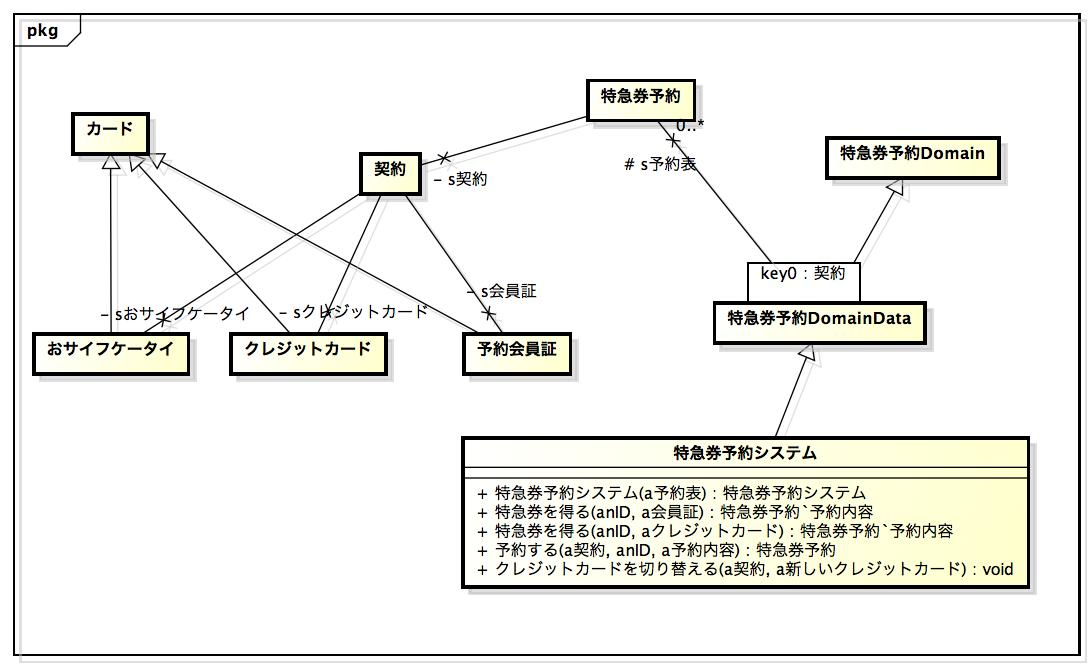
\includegraphics[width=55zw, keepaspectratio] {../EvolvedExpressReservation/image/ModifiedClassDiagram.jpg}}
%			\caption{修正後のクラス図}
%			\label{fig:ModifiedClassDiagram}
%			\index{しゆせいこのくらすす@修正後のクラス図}
%		\end{figure}
%
%		修正後のクラス図は、図\ref{fig:ModifiedClassDiagram}を参照のこと。

\subsection {特急券予約システムモデル化の統計情報}
\addcontentsline{toc}{section}{特急券予約システムモデル化の統計情報}
	\index{とっきゅうけんよやくしすてむもでるかのとうけいじょうほう@特急券予約システムモデル化の統計情報}
注釈抜きのVDM++ソース行数は、501行、
モデル作成工数は約1日、発表用の資料作成とVDM++モデルの読みやすさのための整形・清書に約2日、
モデルの修正工数は1日かかった。

なお、上記モデルの作成工数は、筆者が問題を解決するために消費した工数より少ない。
\chapter {まとめ}
	\label{Conclusion}
		ここまで、なぜ形式手法か?、VDMの概要・成果・導入方法、如何にして対象をモデル化するか?を説明してきたが、
	本章では、ここまで説明した内容を、
	形式手法とVDMの有用性、構造化日本語仕様としてのVDM++という観点からまとめる。

\section{形式手法とVDMの有用性}
	\label{FMEfficency}
	\index{けいしきしゅほうとVDMのゆうようせい@形式手法とVDMの有用性}

	\begin{itemize}
	\item 理論的にも経験的にも形式手法が有効 \\
		証明やモデル検査は、長期的にはやるべきだが、開発現場で導入するのはすぐには難しい。
	\item 証明やモデル検査と比べ、VDM導入はさほど難しくない
		\begin{itemize}
		\item 成功プロジェクト
			\footnote{厳密な仕様記述における形式手法成功事例調査報告書
				(\url{http://sec.ipa.go.jp/reports/20130125.html})
				のTradeOneとFeliCaファームウェアのプロジェクト参照のこと。}
			は、3ヶ月程度の教育とコンサルティングで導入している
		\item 形式手法だけでなく、既存の役立つソフトウェア工学ツールと協調して、より効果が出る
		\end{itemize} 
	\item モデル化は、以下が重要である
		\begin{itemize}
		\item モデル化の範囲を決め、仕様を階層と分割によって、分割統治する
		\item 名詞から型、述語から関数または操作を導き出す
		\item 陰仕様を作成してから、静的検証を行う \\
			この段階で、間違いに気付くことが非常に多い。
		\item 陽仕様を作成してから、動的検証を行う \\
			回帰テストと組合せることで、仕様の変更が容易になる。
		\end{itemize} 
	\item VDM++ソースは、識別子の日本語表現を適切に行うと、構造化日本語仕様として使うことができる
	\end{itemize} 

\section{構造化日本語仕様としてのVDM}
	\label{VDMAsStructuredJapanese}
	\index{こぞうかにほんごとしてのVDM@構造化日本語仕様としてのVDM}

	\ref{ExpressReservationSystem}節\ref{Reserve}段落の操作は、以下のようであり、若干のVDM++知識があれば、
	構造化された日本語仕様として読むことができる。

\begin{verbatim}
public 予約する :  契約 * ID * クレジットカード * 特急券予約`予約内容 ==> 特急券予約
予約する(a契約, anID, aクレジットカード, a予約内容) == (
   def w特急券予約 = new 特急券予約(anID, aクレジットカード, a予約内容) in (
   if 予約がある契約である(a契約, s予約表) then
      s予約表 := 予約表を更新する(s予約表, a契約, w特急券予約)
   else
      s予約表 := 予約表に追加する(s予約表, a契約, w特急券予約);
   return w特急券予約
   )
)
post
   if 予約がある契約である(a契約, s予約表~) then
      予約表が更新されている(s予約表~, a契約, RESULT, s予約表)
   else
      予約表に追加されている(s予約表~, a契約, RESULT, s予約表);
\end{verbatim}

このVDM++仕様から、
事後条件として、
「予約がある契約である」ならば、「予約表が更新されている」状態になり、
そうでなければ、「予約表に追加されている」状態になる
事が分かる。
「予約表が更新されている」ことと「予約表に追加されている」ことの違いは、
それぞれの関数の内容を確認すれば理解できる。

VDM++の知識が少しあれば、
パラメータとして「予約表が更新されている」と「予約表に追加されている」ものに、
インスタンス変数であるs予約表の旧値(old value)と現在の値が渡されていて、
恐らくそれぞれの関数の中で両者の比較が行われていることも分かるし、
返り値を表す予約後のRESULTがパラメータとして渡されることから、
返り値と何かを比較しているだろうことも分かる。

表\ref{PseudocodeVsVDM}に、開発現場でよく使われる、
擬似コードを交えた日本語仕様と適切な日本語を使って構造化されたVDM++仕様の比較を示す。

\begin{table}[h]
	\caption[日本語の仕様中の擬似コードと、VDMの比較]{日本語の仕様中の擬似コードと、VDMの比較}
	\index{にほんごしようちゅうのぎじこーどとVDMのひかく@日本語の仕様中の擬似コードと、VDMの比較}
	\label{PseudocodeVsVDM}
	\begin{center}
		\setlength{\tabcolsep}{3pt}
		\begin{tabular}{|p{5zw}|p{11zw}|p{8zw}|p{9zw}|p{11zw}|p{6zw}|} \hline
			 & 構文を考える時間 & 構文チェック & 関連チェック & 実行テスト & 証明課題生成  \\ \hline\hline
			擬似コードによる仕様  & かなりの時間が必要で、記法も統一できない & レビューのみ & レビューのみ & 
				具体的データを想定したコードインスペクションに相当するチェックのみ(通常行われない) & 不可能 \\ \hline
			VDM仕様  & 言語マニュアルを参照すれば良いだけ & ツールでチェック & ツールの型チェック & 
				ツールで実行 & ツールで生成 \\ \hline
		\end{tabular}
	\end{center}
\end{table}

	表\ref{PseudocodeVsVDM}を見れば、擬似コードを混じえた日本語仕様は「使えない」ことが分かる。

	適切な日本語仕様を使って構造化されたVDM++仕様、
	すなわち構造化日本語仕様としてのVDM仕様は、以下の特徴を持つ。

	\begin{itemize}
	\item 構文を考える時間が不要である \\
		逆に、擬似コードを使う日本語仕様では、
		仕様の意味を考えねばならないのに、構文を考えていることが非常に多い。
	\item 構文・型チェック、証明課題レビューで静的に検証できる \\
		非常に多くの単純ミスを簡単に発見できる。
	\item 証明課題で生成される条件式から、見落としていた不変条件や事前条件が見つかる
	\item 組合せテストにより、動的に正当性検証ができる
	\item 回帰テストにより、動的に妥当性確認ができる
	\item VDMソース自体が、要求辞書ともなる
	\item 日本語仕様より、記述と検証の工数が少ない \\
		特に、仕様修正に強い
	\item 擬似コード形式の日本語仕様に近い形で、かなりの部分を記述できる
	\end{itemize} 

\section{形式手法導入のコツ}
	\label{How2UseFM}
	\index{けいしきしゅほうどうにゅうのこつ@形式手法導入のコツ}

	ここまで説明してきたことから、形式手法導入のコツは極めて簡単であることが分かる。

	すなわち、日本で最大規模の形式仕様記述を使ってプロジェクトを成功に導いた、
	フェリカネットワークスの栗田太郎氏が述べているように、「やれば良いだけです」。
	本書が、そのお役に立てることを願っている。
\chapter {演習問題}
	\label{Exercise}
本章では、演習問題として以下で説明する図書館システムの例題をあげる。

この図書館システムは、どなたでも基本的な機能を理解でき、
規模も非常に小さいが、
我々が開発するシステムの仕様としての基本的な特徴を持っているからである。

\section {図書館システム}
	\label{LibraryRequirement}
	\index{としょかんしすてむ@図書館システム}
	\index{としょかんしすてむへのようきゅう@図書館システムへの要求}
以下の機能を持つ図書館システムを、VDM++でモデル化する。

\begin{enumerate}
\item 本を図書館の蔵書として追加、削除する。
\item 題名と著者と分野のいずれかで本を検索する。
\item 利用者が、蔵書を借り、返す。
\item 蔵書の追加・削除や、利用者への貸出・返却は職員が行う。
\item 利用者や職員の権限などは考慮しなくてよい。
\item 最大蔵書数は10000、利用者一人への最大貸出冊数は3冊とする。
\end{enumerate}

このシステムを、\ref{How2Intro}章と\ref{How2MakeModel}章で説明した方法でモデル化してみよう。

最初にユースケースレベルの要求仕様を作成する。
	\index{ゆーすけーすれべるのようきゅうしよう@ユースケースレベルの要求仕様}
実行不可能だが静的検証のできる陰仕様を作成し、
次に実行可能で動的検証のできる陽仕様を作成し、回帰テストによりテストせよ。

次に、設計仕様を、VDM++を使ったオブジェクト指向モデルとして作成せよ。

解答例は、\ref{LibraryModel}章に示す。

\part {モデルの具体例}
	\label{ModelExamples}

\chapter {演習問題解答の図書館システムモデル}
	\label{LibraryModel}
%\section {図書館0ビジネスロジック}
	\include{libraryByMap/Library0.vpp}
	\include{libraryByMap/Library0RQ1.vdmpp}

%\section {図書館1ビジネスロジック}
	\include{libraryByMap/Library1.vpp}
%\section {図書館1要求辞書}
	\include{libraryByMap/LibraryRQ1.vdmpp}
%\section {図書館1回帰テストケース}
	\include{libraryByMap/MyTest.vpp}
	\include{libraryByMap/MyTestCase.vpp}

%\section {図書館2ビジネスロジック}
	\include{libraryByMap/Library2.vpp}
%\section {図書館2要求辞書}
	\include{libraryByMap/Author2.vdmpp}
	\include{libraryByMap/Book2.vpp}
	\include{libraryByMap/BookStacks.vdmpp}
	\include{libraryByMap/Field2.vdmpp}
	\include{libraryByMap/Lend2.vdmpp}
	\include{libraryByMap/Person2.vdmpp}
	\include{libraryByMap/Staff2.vdmpp}
	\include{libraryByMap/User2.vdmpp}
%\section {図書館2回帰テストケース}
	\include{libraryByMap/MyTest2.vpp}
	\include{libraryByMap/MyTestCase2.vpp}
	\section{\ref{LibraryModel}章の参考文献}
		VDM++\cite{SCSK2012PP}は、
		1970年代中頃にIBMウィーン研究所で開発されたVDM-SL\cite{SCSK2012SL}を拡張し、
		さらにオブジェクト指向拡張した形式仕様記述言語である。


		VDM++の教科書としては\cite{Sakoh2010}がある。

		VDM++を開発現場で実践的に使う場合の解説が\cite{Sahara2008}にある。

\chapter {運賃計算モデル}
	\label{FareModel}
	\include{Fare/CalcFare.vdmpp}
	\include{Fare/FareTableDic.vdmpp}
	\include{Fare/railway_network.vdmpp}
	\include{Fare/route_search.vdmpp}
	\include{Fare/route_search_by_dijkstra.vdmpp}
	\include{Fare/dijkstra.vdmpp}
%\include{Fare/dijkstra4railway.vdmpp}
	\include{Fare/railway_network_data.vdmpp}
	\include{Fare/MyTest.vdmpp}
	\include{Fare/MyTestCase.vdmpp}
%\include{Fare/route_search_testspec.vdmpp}

\chapter {特急券予約システム改善モデル}
	\label{EvolvedExpressReservation}
	\section {発端}
鉄道会社Aの特急券予約システムで特急券を2枚予約し、
以下のような「事件」が起こったのが本モデルを書いた理由である。


以下のやりとりは、電話でのやりとりをかなり(主として用語を中心として)整理したものである。
実際には、例えば、鉄道会社Aサポートセンターの担当者は「カード」という言い方をするのだが、
それがクレジットカードの場合と、予約会員証の場合と、ICカードあるいは予約カードの場合があったので、
個々の用語の正確な名前と意味を調べるだけで
かなりの日数と時間を要した問答であった。

ICカードと予約カードは、結局、この問題とは直接は関係なかったので、この後、本稿に登場することはない。

\begin{itemize}
\item おサイフケータイ(鉄道会社B)で特急券予約システム(鉄道会社A)を使っていた
\item ロンロンViewカードが廃止になりアトレクラブViewカードに変更して下さいとの連絡があった
\item 予約できなかったので 鉄道会社Aサポートセンターに電話

	\begin{description}
	\item [客]「特急券を2枚予約しようとしたが、予約できなかったんですが?」
	\item [JR]「カードを変更したら、特急券予約システムを新規に契約して下さい。」
	\item [客]「新規にすると会費がかかるのでは?」
	\item [JR]「はい。」
	\item [客]「カード会社の都合で変更するのに、それはおかしいでしょう?」
	\item [JR]「では、無料にします。」
	\end{description}

\item 特急券に引換えできなかったので 鉄道会社Aサポートセンターに電話

	\begin{description}
	\item [客]「新しい予約はできたんですが、クレジットカード変更前に予約した特急券に引換えようとしたらできないのですが?」
	\item [JR]「予約会員証で引換できるようになったので、それで引換えて下さい。
			暗証番号はクレジットカードのものを使って下さい。」
	\end{description}

\item T駅での問答

	\begin{description}
	\item [客]「会員証で特急券に引換えできないのですが?」
	\item [JR]「会員証で引換えできないですねー。おかしいな。クレジットカードでやってみましょう。駄目ですねー。」
	\item [客]「古いクレジットカードでは駄目ですか?」
	\item [JR]「あ、できましたね。はい、切符です。」
	\end{description}

\end{itemize} 


\section {モデル化の範囲}
この問題で登場する用語には以下がある。

\begin{itemize}
\item 鉄道会社A、鉄道会社B
\item おサイフケータイ
\item 特急券予約システム
\item 予約会員証、ICカード、予約カード
\item クレジットカード
	\begin{itemize}
	\item ロンロンViewカード、アトレクラブViewカード
	\end{itemize} 
\item 特急券
\end{itemize} 

「鉄道会社B」「ICカード」「予約カード」は、モデルを単純化するため対象としなかった。

「鉄道会社A」の「特急券予約システム」システムのうち、
以下の機能だけをVDM++\cite{SCSK2012PP}で要求仕様としてモデル化し、
問題点を明確化することにした。

\begin{itemize}
\item 予約する
\item 特急券を得る
\item クレジットカードを切り替える
\end{itemize} 

従って、モデル化する範囲に登場するpublicな用語は以下だけである。
\begin{itemize}
\item おサイフケータイ
\item 特急券予約システムシステム
\item 特急券予約システム
\item 予約会員証
\item クレジットカード
\item 特急券
\end{itemize} 





	
	\include{EvolvedExpressReservation/ReservationSysytem.vpp}	
	\include{EvolvedExpressReservation/Common.vpp}
	\include{EvolvedExpressReservation/ReservationDomain.vpp}
	\include{EvolvedExpressReservation/ReservationDomainData.vpp}
	\include{EvolvedExpressReservation/ExpressReservatiopn.vpp}
	\include{EvolvedExpressReservation/Contract.vpp}
	\include{EvolvedExpressReservation/Card.vpp}
	\include{EvolvedExpressReservation/CredirCard.vpp}
	\include{EvolvedExpressReservation/CustomerCard.vpp}
	\include{EvolvedExpressReservation/Wallet.vpp}
	\include{EvolvedExpressReservation/MyTest.vpp}
	\include{EvolvedExpressReservation/MyTestCase.vpp}
	\subsubsection{まとめ}
\paragraph{問題は何だったのか?}
結局、問題は何だったのかといえば、
特急券予約システムのクレジットカードによる決済のモデルが考慮不足だったということになる。

まず、おサイフケータイのクレジットカードを変更すると、
特急券予約システムを新規に契約せねばならず、
予約会員証も新規に作成しなければならない。

しかし、変更前の予約を行った古いクレジットカードは、
その予約の特急券を受け取るときに必要になる。
何故なら、クラス図\ref{fig:ExpressReservationClassDiagram}で見るように、
個々の予約を表す特急券予約システムからクレジットカードにリンクが設定されているからである。

\begin{figure}[h]
	\centering
	{\includegraphics[width=55zw, keepaspectratio]{./image/ClassDiagram.jpg}}
	\caption{クラス図(特急券予約システム)}
	\label{fig:ExpressReservationClassDiagram}
	\index{くらすすとっきゅうけんよやくしすてむ@クラス図(特急券予約システム)}
\end{figure}

このような構造でも、変更後にすべての特急券予約システムからクレジットカードへのリンクを
新しいクレジットカードに変更していれば問題はないはずだが、
恐らく、変更に掛かる効率を理由に、古いクレジットカードとリンクしたままになっているのであろう。
設計上の理由で、ユーザーに迷惑を掛ける仕様となっている訳である。

さらに、モデルに問題があった。
予約会員証は新規に作るのが普通であるが、
クレジットカード会社の都合による変更のため、
新規に契約する費用は無料となった。
そのため、予約会員証は古いものを使用することになった。
契約は新規だが、予約会員証は古く、
そしてクラス図\ref{fig:ExpressReservationClassDiagram}から分かるように、
予約会員証からリンクしているクレジットカードは、
変更前の古いものであるという訳である。

これではまずいと思って、鉄道会社Aの係員がリンクされているクレジットカードを新しいものにしたようである。
その結果、変更前の特急券予約システムを予約会員証で特急券を得ることができなかった。


\paragraph{本来どうすべきだったのか?}
本来、特急券予約システムは契約\footnote{口座と言ってもよいが、本モデルでは契約という名前にした}
とリンクが設定されているべきであり、
契約がクレジットカードとリンクしているべきである。

予約会員証も契約を介してクレジットカードを参照できるようにすべきである。

このようにしておけば、契約に変更があっても、古い特急券予約システムは新しい契約を介して、新しいクレジットカードにアクセスでき、
同じく予約会員証も新しいクレジットカードにアクセスできる。

本来どうすべきだったのかを検証するVDM++モデルは、1日で記述および検証ができた。

詳細は、「特急券予約システムシステムの問題点を推測し、修正した仕様」を参照のこと。


\paragraph{統計情報}
注釈抜きのVDM++ソース行数は、492行、
モデル作成工数は約1日、発表用の資料作成とVDM++モデルの読みやすさのための整形・清書に約2日かかった。

なお、上記モデルの作成工数は、筆者が問題を解決するために消費した工数より少ない。


%\section {ユーティリティ SSlib}
%\include{libraryByMap/Character.vpp}
%\include{libraryByMap/Sequence.vpp}
%\include{libraryByMap/String.vpp}

%\newpage
%\layout

%\begin{thebibliography}{9}

\bibliographystyle{jplain}
%\bibliography{/Users/sahara/svnw/sahara}
\bibliography{/Users/sahara/Dropbox/bib/saharaUTF8}
%\bibliography{/Users/ssahara/svnwork/sahara}

%\end{thebibliography}

\newpage
\printindex

\end{document}
